\documentclass[11pt]{article}
\usepackage[a4paper,margin=1in]{geometry}
\usepackage{amsmath,amssymb,amsthm,mathtools}
\usepackage[expansion=false]{microtype}
\usepackage{graphicx,booktabs,array}
\usepackage[font=small,labelfont=bf]{caption}
\usepackage[dvipsnames]{xcolor}
\usepackage{enumitem}
\usepackage[hidelinks,pdfusetitle]{hyperref}
\usepackage[nameinlink,capitalise]{cleveref}
\setlist{nosep,leftmargin=1.5em}
\newtheorem{theorem}{Theorem}
\newtheorem{lemma}[theorem]{Lemma}
\newtheorem{proposition}[theorem]{Proposition}
\newtheorem{corollary}[theorem]{Corollary}
\theoremstyle{definition}\newtheorem{definition}[theorem]{Definition}
\theoremstyle{remark}\newtheorem{remark}[theorem]{Remark}
\newcommand{\R}{\mathbb R}\newcommand{\C}{\mathbb C}\newcommand{\N}{\mathbb N}
\newcommand{\dd}{\,\mathrm d}\newcommand{\e}{\mathrm e}
\newcommand{\Num}{\mathrm{Num}}\newcommand{\Den}{\mathrm{Den}}
\renewcommand{\Re}{\operatorname{Re}}\renewcommand{\Im}{\operatorname{Im}}
\setlength{\parskip}{0.35em}
\AtBeginDocument{\sloppy}
\urlstyle{same}
\hypersetup{pdftitle={Which Member Carries: Two-State Pairs from Atoms to Gas Sensors, and Doebereiner's Triads as Balanced Pairs},pdfauthor={Abhijit Singh}}
\title{\textbf{Which Member Carries:}\\[4pt]
\large Two-State Pairs from Atoms to Gas Sensors, and D\"obereiner's Triads as Balanced Pairs}
\author{Abhijit Singh}
\date{25 September 2026}
\begin{document}
\maketitle
\begin{abstract}
Which member of a pair carries (the charge, the population, the change of nuclear charge, the electron of a sensor surface, the centre of a triad) is decided in chemistry by one law, the two-state pair $p=1/(1+e^{\varepsilon})$ split into a common part $\frac12$ and a difference $\delta=-\frac12\tanh(\varepsilon/2)$. We show that an observation of which member carries determines $\delta$ and nothing else, and we evaluate the pair in six settings. Potassium carries the charge of the separated pair Na, K at every temperature: the minority configuration $\mathrm{Na^+}+\mathrm K$ has occupancy $3.87\times10^{-14}$ at 300 K as a single pair and $1.97\times10^{-7}$ in an equimolar gas, where mass action halves the exponent. The mean nuclear charge change per decay of ${}^{40}$K is $+0.7856(22)$ from the 2017 ENSDF evaluation and $+0.7918(10)$ from the 2023 KDK branching ratios, $2.6$ combined standard uncertainties apart. The upper fine-structure level of aluminium holds the majority above $T_{1/2}=232.61$ K. We prove that a code shared by the absent rows of two channels turns their correlation exactly into $(r+fd_xd_y)/\sqrt{(1+fd_x^2)(1+fd_y^2)}$, whose sign flips when the geometric-mean code distance crosses $\sqrt{-r/f}$; from the present-row moments of two sensor channels of the UCI air-quality record this closed form reproduces the coded correlations $+0.086931$ (code $-200$, geometric-mean distance $4.9133$) and $-0.075630$ (code $0$, distance $4.0595$) to $10^{-16}$.

First-order mass action makes the ionosorbed-oxygen occupancy of a metal-oxide surface an exact logistic in $\varepsilon=\ln(\Phi_+/\Phi_-)$, the log-ratio of the electron-release and electron-trapping fluxes. Fitted to the five sensors of the same record on the common CO axis, the two-state law is preferred to the offset power law for every sensor ($\Delta\mathrm{AIC}=11.7$ to $209.0$), with slopes $\beta=1.18$ to $1.45$, and it orders the sensors into a ladder of half-points: S3 ($1.68$ mg\,m$^{-3}$, the falling tungsten-oxide surface, which reads the opposite member) $<$ S5 ($4.61$) $<$ S2 ($5.40$) $<$ S1 ($7.49$, at the upper edge of the data) $<$ S4 (not identified), with S3 $<$ S5 $<$ S2 in both halves of the year. Humidity enters every sensor on the side of the reducing gas. In this urban record NO$_2$ rises with CO, so the oxidizing member is not separable through NO$_2$; the opposite-sign pair is CO against NO on S4, with balance slope $3.28$. The record's benzene column is an exact power law of the titania sensor, $1.23978\times10^{-4}(S_2-324.785)^{1.743158}$ to $1.6\times10^{-15}$: a calibration output, not a measurement. From the Madelung order we prove the period-pair law $L(p)=2\lceil(p+1)/2\rceil^2$ and that a vertical triad is exact, $Z_2=\frac12(Z_1+Z_3)$, if and only if the two periods it spans have equal length. Of the 54 vertical triads, 27 are exact, including all four of D\"obereiner's; their middle member is the zero of the pair $(-s,+s)$, $s\in\{8,18,32\}$. The same mass-action pair decides which gas survives the NH$_4$SH deck of the giant planets. The proofs solve the steady state of first-order mass action, decompose pooled moments and count subshells in the Madelung order; the sensor results are least-squares fits with day-block bootstrap intervals.
\end{abstract}

\section{Introduction}\label{sec:intro}
D\"obereiner observed in 1829 that chemically similar elements come in threes whose middle atomic weight is close to the mean of the other two \cite{Dob1829}. Scerri recast such triads in terms of atomic number, where the middle value can be the exact mean, and used them to compare the medium-long and left-step forms of the periodic table \cite{Scerri2008,Scerri2010,Scerri2022}; the lengths of the periods follow the Madelung $(n+\ell,n)$ order, whose origin Allen and Knight discuss \cite{AllenKnight}. The branching of ${}^{40}$K between $\beta^-$ decay and electron capture has two recent determinations, the 2017 ENSDF evaluation \cite{Chen} and the 2023 KDK measurement of ground-state capture \cite{KDK,Kossert}. For metal-oxide gas sensors the ionosorption model \cite{BarsanWeimar2001,MadouMorrison} and the depletion theory of Yamazoe and Shimanoe \cite{YamazoeShimanoe} account for the empirical power laws, and the air-quality record of De Vito et al.\ \cite{DeVito,UCI}, a year of hourly readings of five such sensors beside reference analysers, is a standard record for their field calibration. For tables with absent values, the attenuation of correlations by imputation is known qualitatively \cite{LittleRubin,SchaferGraham}.

We treat all of these as one pair. A pair of states with weights $(p,1-p)$ can be written without loss as a common part and a difference,
\begin{equation}\label{eq:pair}
p=\tfrac12+\delta,\qquad1-p=\tfrac12-\delta,\qquad\delta=-\tfrac12\tanh(\varepsilon/2),\qquad\varepsilon=\ln\frac{1-p}p .
\end{equation}
Indeed $\varepsilon=\ln((1-p)/p)$ inverts to $p=1/(1+e^{\varepsilon})$, and then $p-\frac12=(1-e^{\varepsilon})/(2(1+e^{\varepsilon}))=-\frac12\tanh(\varepsilon/2)$. The log-odds $\pm\varepsilon$ form a pair whose zero $\varepsilon=0$ is located in turn at a temperature, a code distance, a gas concentration and a middle atomic number; independent adsorption sites and independent products of a charge transfer combine without changing the law; an exact vertical triad of the periodic table is $Z_2+\{-s,0,s\}$; and an observation of which member carries determines $\delta$ and nothing else, since every factor common to the two members cancels, while in a group the shared end of two exact triads closes the first and opens the next.

\paragraph{Companion papers.} The same law with $\varepsilon=-z(V-V_{1/2})$ is the gate law of excitable membranes \cite{Neuro}: there the half-point is a voltage, and for a gate moving an effective charge through the membrane field $\varepsilon$ is again a free-energy difference in units of $k_BT$. The same mass-action pair decides the top ice deck of the giant planets \cite{Planet} (\cref{sec:giants}). An exact triad $Z_2+s\{-1,0,1\}$ is the digit set of balanced ternary scaled by $s$; the arithmetic and radix economy of that digit set are treated in \cite{Algo}. The synthesis paper \cite{Synth} places these results beside those of the other fields.

\subsection{Main results}\label{sec:main}
Our main results are the following.
\begin{enumerate}[label=(\arabic*)]
\item \emph{The pair and its half-point} (\cref{sec:half}). Every two-state distribution is the pair \eqref{eq:pair}, whose difference $\delta$ is odd under the exchange $\varepsilon\mapsto-\varepsilon$ of the members. A pair with degeneracies $g_l$, $g_u$ and gap $\Delta E>0$ balances at a positive temperature if and only if $g_u>g_l$, and then exactly at $T_{1/2}=\Delta E/(k_B\ln(g_u/g_l))$ (\cref{prop:half}).
\item \emph{Sodium and potassium} (\cref{sec:nak}). One valence electron shared between a sodium and a potassium core is carried by potassium at every temperature: the configurations $\mathrm{Na}+\mathrm K^+$ and $\mathrm{Na}^++\mathrm K$ lie $0.7984132(3)$ eV apart with degeneracy ratio $1$, so balance is unreachable. The minority configuration has occupancy $3.87\times10^{-14}$ at 300 K as a single pair and $1.97\times10^{-7}$ in an equimolar gas, where the two products form independently and mass action halves the exponent.
\item \emph{The two branches of ${}^{40}$K} (\cref{sec:k40}). The mean nuclear charge change per decay is the difference of the pair, $\langle\Delta Z\rangle=\tanh(\varepsilon/2)=2p_{\beta^-}-1$. It is $+0.7856(22)$ from the 2017 ENSDF evaluation and $+0.7918(10)$ from the 2023 KDK branching ratios; the two differ by $0.0062$, that is by $2.6\sigma$, with $\sigma=0.0024$ the combined standard uncertainty.
\item \emph{The fine-structure doublet of aluminium} (\cref{sec:al}). The upper level ${}^2P^\circ_{3/2}$ ($g=4$, $112.061\ \mathrm{cm^{-1}}$) holds the majority above $T_{1/2}=232.61$ K and tends to $\frac23$.
\item \emph{Joint absences} (\cref{sec:code}). If two channels with present-row correlation $r$ are absent together on a fraction $f$ of the rows and these rows carry a shared code at standardised distances $d_x$, $d_y$ from the present-row means, their correlation is exactly
\[
r_{\mathrm{coded}}=\frac{r+f\,d_xd_y}{\sqrt{(1+fd_x^2)(1+fd_y^2)}};
\]
for $r<0$ and $d_xd_y>0$ its sign flips when the geometric-mean distance $\sqrt{d_xd_y}$ crosses $\sqrt{-r/f}$, however unequal $d_x$ and $d_y$ are, and one coded correlation bounds how far its code lies from the data (\cref{prop:code}). From the present-row moments of the sensors PT08.S1 and PT08.S3 of the UCI air-quality record this closed form reproduces exactly the coded correlations of the record, $+0.086931$ for the code $-200$ ($\sqrt{d_xd_y}=4.9133$) and $-0.075630$ for the code $0$ ($4.0595$), to $10^{-16}$; the flip lies between them, at $4.4424$.
\item \emph{The two-state law of a sensor surface, and the sensor ladder} (\cref{sec:sensor}). First-order mass action makes the ionosorbed-oxygen occupancy of a metal-oxide grain the exact logistic $\theta=1/(1+e^{\varepsilon})$ with $\varepsilon=\ln(\Phi_+/\Phi_-)$, the log-ratio of the electron-release and electron-trapping fluxes (\cref{prop:mos}). Fitted to the five sensors of the air-quality record on the common CO axis, the two-state law is preferred to the offset power law for every sensor ($\Delta\mathrm{AIC}=11.7$ to $209.0$), with slopes $\beta=1.18$ to $1.45$ near first-order mass action, and its half-points form the ladder
\[
\text{S3 }(1.68)\ <\ \text{S5 }(4.61)\ <\ \text{S2 }(5.40)\quad\mathrm{mg\ m^{-3}}\ \text{of CO},
\]
identified inside the data and ordered in the same way in both halves of the year, with S1 ($7.49$) at the upper edge of the data and S4 not identified. The tungsten-oxide sensor S3 falls with every traffic gas: it reads the opposite member of the same pair. Humidity enters every sensor on the side of the reducing gas. In this urban record NO$_2$ rises with CO, so the CO and NO$_2$ coefficients carry the same sign on S1, S2, S3 and S5 and the oxidizing member is not separable through NO$_2$; the opposite-sign pair appears as CO against NO on S4, with balance slope $3.28$ [$2.90$, $3.73$].
\item \emph{The benzene column} (\cref{sec:benzene}). The column C$_6$H$_6$(GT) of the record is the exact power law $1.23978\times10^{-4}(S_2-324.785)^{1.743158}$ of the titania sensor S2 on all 8991 rows, to a relative deviation of $1.6\times10^{-15}$. It is a calibration output, not an independent measurement, and its form is the power-law regime of the two-state law.
\item \emph{The period-pair law and D\"obereiner's triads} (\cref{sec:pair,sec:triads,sec:props}). Period $p$ has the capacity of the Madelung group $n+\ell=p+1$, so $L(p)=2\lceil(p+1)/2\rceil^2$ (\cref{prop:pair}). A vertical triad is exact, $Z_2=\frac12(Z_1+Z_3)$, if and only if the two periods it spans have equal length (\cref{thm:exact}). Of the 54 vertical triads, 27 are exact; their middle member is the zero of the pair $(-s,+s)$, $s\in\{8,18,32\}$. D\"obereiner's four triads are all exact, Li--Na--K with $s=8$ and Ca--Sr--Ba, Cl--Br--I and S--Se--Te with $s=18$; their middle atomic weights lie $0.13$ to $1.57\%$ below the mean of the outer pair, and in all six exact triads of groups 1, 2, 16 and 17 the middle first ionization energy lies strictly between the outer two.
\item \emph{The giant planets} (\cref{sec:giants}). The mass-action pair of the sensor surface also decides the top ice deck of the giant planets: NH$_3$ and H$_2$S are titrated 1:1 by the NH$_4$SH lattice, their difference $x_{\mathrm N}-x_{\mathrm S}=2\chi\sinh(\varepsilon/2)$ is conserved, and the surviving vapour is $\operatorname{sign}(N-S)$, so the zero $N/S=1$ separates Jupiter ($4.73$) and Saturn ($3.16$) from Uranus ($0.195$) and Neptune ($0.170$) \cite{Planet}.
\end{enumerate}

\subsection{Outline of the method}
The exact statements come from first-order mass action and from counting. \Cref{prop:half,prop:mos} solve the steady state of a two-state balance and read off its zero. \Cref{prop:code} decomposes the pooled moments of a coded table into present-row moments and code distances, and its bound is the Cauchy--Schwarz inequality; \cref{prop:mcar} does the same for mean imputation. \Cref{prop:pair} counts the subshells of each Madelung group, and \cref{thm:exact} compares the gaps down a group with the period lengths through an alignment lemma (\cref{lem:align}). The atomic and nuclear results evaluate these formulas on tabulated data. The sensor results fit the two-state law to the hourly record by nonlinear least squares, compare it with the offset power law through the Akaike criterion, and take 95\% intervals from a bootstrap that resamples whole days, so that the serial correlation of hourly data is respected (\cref{sec:stat}).

\subsection{Organisation and notation}
\Cref{sec:half} treats the pair and its half-point, \cref{sec:nak,sec:k40,sec:al} the three evaluated atomic and nuclear pairs, \cref{sec:code} the coding of absent measurements, \cref{sec:sensor} the sensor ladder, the benzene column and the giant planets, \cref{sec:pair,sec:triads,sec:props} the periodic table, and \cref{sec:explore} horizontal triads and lanthanide-contraction pairs; \cref{sec:summary} concludes, and \cref{sec:data} lists every input. Throughout, $p$ is the occupancy of a member, $\varepsilon$ its log-odds against the other and $\delta=p-\frac12$ the difference; $T_{1/2}$, $d^*$ and $C_{1/2}$ are the zeros $\varepsilon=0$ in temperature, code distance and concentration; $k_B$ is the Boltzmann constant. For the periodic table, $L(p)$ and $\Sigma(p)$ are the length and the last atomic number of period $p$, and $\eta=x_2/\bar x-1$ is the deviation of a middle member from the mean $\bar x$ of the outer pair. Numbers in square brackets after an estimate are 95\% day-block bootstrap intervals.

\section{The pair and its half-point}\label{sec:half}
In the pair \eqref{eq:pair} the common part $\frac12$ says nothing about which member is favoured; the difference $\delta$ says everything, and it is odd under $\varepsilon\mapsto-\varepsilon$, the exchange of the two members. For a two-state system in thermal equilibrium $\varepsilon$ is the free-energy difference in units of $k_BT$; for competing decay branches it is the logarithm of a ratio of partial decay constants (\cref{sec:k40}); for a sensor surface it is the logarithm of the ratio of the electron-release and electron-trapping fluxes (\cref{sec:mos}).

If the two members have degeneracies $g_l$, $g_u$ and energy separation $\Delta E>0$, the upper member's occupancy is
\[
p_u(T)=\frac{g_ue^{-\Delta E/k_BT}}{g_l+g_ue^{-\Delta E/k_BT}},\qquad\varepsilon(T)=\frac{\Delta E}{k_BT}-\ln\frac{g_u}{g_l}.
\]
\begin{proposition}\label{prop:half}
The pair is balanced ($p_u=\frac12$) at a positive temperature iff $g_u>g_l$, and then exactly at $T_{1/2}=\Delta E/(k_B\ln(g_u/g_l))$; as $T\to\infty$, $p_u\to g_u/(g_u+g_l)$. If $g_u\le g_l$ the upper member remains the minority at every temperature. Equivalently, the upper member is the majority at temperature $T$ iff $\Delta E<k_BT\ln(g_u/g_l)$.
\end{proposition}
\begin{proof}
Dividing numerator and denominator by $g_ue^{-\Delta E/k_BT}$ gives $p_u=1/(1+e^{\varepsilon(T)})$, so $p_u>\frac12$ iff $\varepsilon<0$ and $p_u=\frac12$ iff $\varepsilon=0$. Since $\Delta E>0$, $\varepsilon(T)$ decreases strictly and continuously from $+\infty$ (as $T\to0^+$) to $-\ln(g_u/g_l)$ (as $T\to\infty$). If $g_u>g_l$ the limit is negative and $\varepsilon$ has exactly one zero, $\Delta E/k_BT=\ln(g_u/g_l)$, i.e.\ $T=T_{1/2}$; if $g_u\le g_l$ the limit is $\ge0$ and $\varepsilon>0$ at every finite $T$. As $T\to\infty$, $p_u\to1/(1+g_l/g_u)=g_u/(g_u+g_l)$. The last statement is $\varepsilon(T)<0$ rewritten.
\end{proof}

\section{One electron, two cores: sodium and potassium}\label{sec:nak}
Consider isolated gas-phase atoms. One valence electron shared between a sodium and a potassium core at large separation (the two lowest dissociation limits of $\mathrm{NaK^+}$) is in one of the configurations $\mathrm{Na}+\mathrm K^+$ or $\mathrm{Na}^++\mathrm K$, separated by the difference of first ionisation energies,
\[
\Delta E=5.13907696(25)-4.34066373(9)=0.7984132(3)\ \text{eV}\quad\text{\cite{NIST,SansonettiMartin}},
\]
with the lower configuration $\mathrm{Na}+\mathrm K^+$: potassium carries the charge. (The uncertainty is the quadrature sum of the two stated uncertainties.) Both neutral atoms are ${}^2S_{1/2}$ and both ions ${}^1S_0$ \cite{SansonettiMartin}, so each configuration has electronic degeneracy $2\cdot1=1\cdot2=2$, the degeneracy ratio is $1$, and by \cref{prop:half} balance is unreachable at every temperature. As a two-state system, $\varepsilon=\Delta E/k_BT$ with $k_B=8.617333262\times10^{-5}$ eV\,K$^{-1}$ \cite{CODATA}, and the minority occupancy is $1/(1+e^{\varepsilon})$:
\begin{center}\small
\begin{tabular}{@{}lccc@{}}\toprule
$T$ (K) & 300 & 310 & 1000\\\midrule
$\varepsilon=\Delta E/k_BT$ & $30.884$ & $29.888$ & $9.265$\\
occupancy of $\mathrm{Na}^++\mathrm K$ & $3.87\times10^{-14}$ & $1.05\times10^{-13}$ & $9.47\times10^{-5}$\\\bottomrule
\end{tabular}
\end{center}
Solving $1/(1+e^{\varepsilon})=p$ for the temperature gives $T=\Delta E/(k_B\ln((1-p)/p))$: the minority configuration reaches $10^{-6}$ at $671$ K and $10^{-3}$ at $1341$ K.

\emph{A pair is not a mixture.} In a gas prepared with equal amounts $c_0$ of $\mathrm{Na}$ and $\mathrm K^+$, consider the charge-transfer equilibrium $\mathrm{Na}+\mathrm K^+\rightleftharpoons\mathrm{Na}^++\mathrm K$. For ideal gases the equilibrium constant is the ratio of the partition functions per unit volume, each with energies measured from its own ground state, $K_{\mathrm{eq}}=(q_{\mathrm{Na}^+}q_{\mathrm K})/(q_{\mathrm{Na}}q_{\mathrm K^+})\,e^{-\Delta E/k_BT}$. The electronic factors cancel (degeneracy $1\cdot2$ on each side), and excited electronic states do not contribute below $1000$ K: the lowest ones, K $4p\,{}^2P^\circ_{1/2,3/2}$ at $12985.19$ and $13042.90\ \mathrm{cm^{-1}}$ ($1.61$ eV) \cite{NIST}, hold a fraction $2.2\times10^{-8}$ of K atoms at $1000$ K, and all other excitations lie higher. The translational factors, proportional to $m^{3/2}$, leave $[(1-m_e/m_{\mathrm{Na}})(1+m_e/m_{\mathrm{K^+}})]^{3/2}=1-1.5\times10^{-5}$, with $m_e=5.486\times10^{-4}$ u \cite{CODATA} and $m\approx23$ u, $39$ u; we set this factor to $1$. With converted fraction $x$ the amounts are $xc_0$ of $\mathrm{Na}^+$ and of $\mathrm K$ and $(1-x)c_0$ of $\mathrm{Na}$ and of $\mathrm K^+$, so $K_{\mathrm{eq}}=x^2/(1-x)^2$ and
\[
\frac{x}{1-x}=e^{-\Delta E/2k_BT},\qquad x=1.97\times10^{-7}\ (300\ \text{K}),\quad 9.64\times10^{-3}\ (1000\ \text{K}).
\]
The exponent is halved because the two products form independently: the single pair and the mixture answer different questions, and the square root is the whole difference between them.

\section{The two branches of \texorpdfstring{${}^{40}$K}{40K}}\label{sec:k40}
${}^{40}$K ($0.0117\%$ of natural potassium \cite{Meija}) decays by $\beta^-$ to ${}^{40}$Ca ($\Delta Z=+1$) or by electron capture (and a $10^{-5}$ fraction of $\beta^+$) to ${}^{40}$Ar ($\Delta Z=-1$). Here $\varepsilon=\ln(\lambda_{\beta^-}/\lambda_{\mathrm{EC}})$ is the logarithm of a ratio of partial decay constants, not a thermal quantity. The branching fractions are $p_{\beta^-}=\lambda_{\beta^-}/(\lambda_{\beta^-}+\lambda_{\mathrm{EC}})=1/(1+e^{-\varepsilon})$ and $p_{\mathrm{EC}}=1-p_{\beta^-}$, where $p_{\mathrm{EC}}$ stands for electron capture together with the $\beta^+$ branch (the column $p_{\mathrm{EC}}+p_{\beta^+}$ of the table below), which also lowers $Z$ by one. The net nuclear charge change per decay is the difference of the pair,
\[
\langle\Delta Z\rangle=(+1)\,p_{\beta^-}+(-1)\,p_{\mathrm{EC}}=\frac{1-e^{-\varepsilon}}{1+e^{-\varepsilon}}=\tanh(\varepsilon/2)=2p_{\beta^-}-1,
\]
whose standard uncertainty is twice that of $p_{\beta^-}$, since the two fractions sum to one. The entropy per decay is $-p_{\beta^-}\log_2p_{\beta^-}-p_{\mathrm{EC}}\log_2p_{\mathrm{EC}}$.
\begin{center}\small
\begin{tabular}{@{}lcccc@{}}\toprule
evaluation & $p_{\beta^-}$ (\%) & $p_{\mathrm{EC}}+p_{\beta^+}$ (\%) & $\langle\Delta Z\rangle$ & entropy (bits/decay)\\\midrule
ENSDF 2017 \cite{Chen} & $89.28(11)$ & $10.72(11)$ & $+0.7856(22)$ & $0.4914$\\
KDK 2023 \cite{KDK,Kossert} & $89.59(5)$ & $10.41$ & $+0.7918(10)$ & $0.4818$\\\bottomrule
\end{tabular}
\end{center}
The KDK entry combines their measured ground-state capture $0.098(25)\%$ (statistical and systematic uncertainties $0.023$ and $0.010$ combined in quadrature) with the capture to the excited state, $10.31(4)\%$, both from their re-evaluation of the decay scheme using the partial decay constants of \cite{Kossert}, and the $\beta^+$ branch $0.001\%$ of \cite{Chen}; the three electron-capture-side entries and $p_{\beta^-}$ sum to $0.99999$ and are normalised to one before $\langle\Delta Z\rangle$ and the entropy are formed. The two values of $\langle\Delta Z\rangle$ differ by $0.0062$, or $2.6$ combined standard uncertainties ($\sqrt{0.0022^2+0.0010^2}=0.0024$). The common part $\frac12$ counts decays; the difference is the charge. A balanced branching would carry no net charge on average and one full bit per decay.

\section{The fine-structure doublet of aluminium}\label{sec:al}
The ground term of neutral aluminium is $3s^{2}3p\,{}^2P^\circ$, with ${}^2P^\circ_{1/2}$ ($g=2$) lowest and ${}^2P^\circ_{3/2}$ ($g=4$) at $112.061\ \mathrm{cm^{-1}}$ \cite{NIST}, i.e.\ $\Delta E/k_B=hc\tilde\nu/k_B=161.231$ K ($13.894$ meV) with the second radiation constant $hc/k_B=1.438776877$ cm\,K \cite{CODATA}; the next level, $3s^{2}4s\,{}^2S_{1/2}$, lies at $25347.756\ \mathrm{cm^{-1}}$ \cite{NIST}. For atoms thermalised at temperature $T$ within the ground-term manifold (for example in a buffer gas), $p_u(T)=2e^{-\Theta/T}/(1+2e^{-\Theta/T})$ with $\Theta=161.231$ K, and \cref{prop:half} with $g_u/g_l=2$ gives
\[
T_{1/2}=\frac{hc\tilde\nu}{k_B\ln2}=232.61\ \text{K},
\]
above which the upper level holds the majority, tending to $\frac23$. Values of $p_u$: $0.198$ (77 K), $0.406$ (150 K), $\frac12$ (232.61 K), $0.539$ (300 K), $0.630$ (1000 K), $0.666$ ($10^5$ K). By the last clause of \cref{prop:half}, a ${}^2P$ ground term with the $J=\frac12$ level lowest has its excited level in the majority at 300 K iff the splitting is below $k_B\cdot300\,\mathrm K\cdot\ln2=144.5\ \mathrm{cm^{-1}}$; aluminium's $112.061\ \mathrm{cm^{-1}}$ qualifies. At $T_{1/2}$ each level holds $\frac12$, so each of the two lower states has probability $\frac14$ and each of the four upper states $\frac18$; the six ground-term states then carry $2\cdot\frac14\log_24+4\cdot\frac18\log_28=1+1.5=2.5$ bits of entropy (the maximum, $\log_26=2.585$ bits, is approached only as $T\to\infty$, where all six states have probability $\frac16$).

\begin{figure}[t]\centering
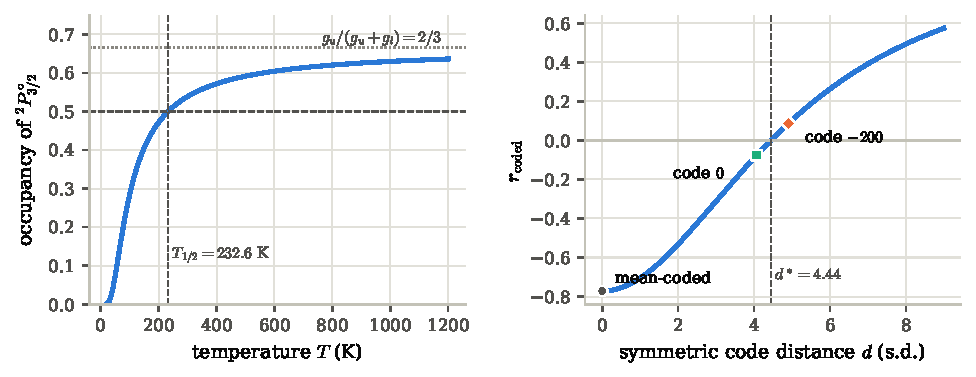
\includegraphics[width=\textwidth]{fig5_pairs.pdf}
\caption{Left: occupancy of Al ${}^2P^\circ_{3/2}$ for atoms thermalised in the ground term; the pair balances at $T_{1/2}=232.6$ K and tends to $g_u/(g_u+g_l)=\frac23$. Right: the symmetric-code curve $G(d)=(r+fd^2)/(1+fd^2)$ of \cref{prop:code} for $r=-0.771918$ and $f=366/9357$ (channels PT08.S1 and PT08.S3 of the air-quality record); the sign flips at $d^*=4.44$. The markers place the coded correlations $+0.0869$ (code $-200$) and $-0.0756$ (code $0$) at their symmetric-equivalent distances $d_{\mathrm{sym}}=4.904$ and $4.068$. The directly computed geometric-mean distances of the two codes, $4.913$ and $4.060$, lie on the sides that \cref{prop:code}(d) requires: above $d_{\mathrm{sym}}$ for $-200$ and below it for $0$.}
\label{fig:pairs}
\end{figure}

\section{The coding of absent measurements}\label{sec:code}
Two channels $X$, $Y$ are recorded on $n$ rows. On the $n_{11}$ rows where both are present they have means $\mu_x,\mu_y$, variances $v_x,v_y>0$ and covariance $c$, all with divisor $n_{11}$, and $r=c/\sqrt{v_xv_y}$. Suppose first that the other $n-n_{11}=fn$ rows, $0<f<1$, are absent in \emph{both} channels and are filled with constants $(a_x,a_y)$. Write the standardised code distances
\[
d_x=\frac{a_x-\mu_x}{\sqrt{v_x}},\qquad d_y=\frac{a_y-\mu_y}{\sqrt{v_y}} .
\]

\begin{proposition}[joint absences]\label{prop:code}
The correlation over all $n$ rows is
\begin{equation}\label{eq:code}
r_{\mathrm{coded}}=\frac{r+f\,d_xd_y}{\sqrt{(1+fd_x^2)(1+fd_y^2)}} .
\end{equation}
(a) (Mean-coding is invisible.) If $d_x=d_y=0$ then $r_{\mathrm{coded}}=r$, the value obtained by deleting the absent rows.
\par\noindent(b) (Sign.) $r_{\mathrm{coded}}$ has the sign of $r+f\,d_xd_y$. If $r<0$ and $d_xd_y>0$ the sign changes exactly when the geometric-mean distance $\sqrt{d_xd_y}$ crosses $d^*=\sqrt{-r/f}$, however unequal $d_x$ and $d_y$ are.
\par\noindent(c) (A shared distant code manufactures agreement.) As $|d_x|,|d_y|\to\infty$, $r_{\mathrm{coded}}\to\operatorname{sign}(d_xd_y)$, whatever $r$ was.
\par\noindent(d) (Bound.) $|r_{\mathrm{coded}}|\le|r+f\,d_xd_y|/(1+f|d_xd_y|)$, with equality iff $|d_x|=|d_y|$. Consequently, if $d_xd_y>0$ and $G(d)=(r+fd^2)/(1+fd^2)$ is the symmetric-code curve, an observed $r_{\mathrm{coded}}$ defines $d_{\mathrm{sym}}\ge0$ by $G(d_{\mathrm{sym}})=r_{\mathrm{coded}}$, i.e.\ $d_{\mathrm{sym}}^2=(r_{\mathrm{coded}}-r)/(f(1-r_{\mathrm{coded}}))$, and
\[
\sqrt{d_xd_y}\ \ge\ d_{\mathrm{sym}}\ \text{ if } r_{\mathrm{coded}}>0,\qquad \sqrt{d_xd_y}\ \le\ d_{\mathrm{sym}}\ \text{ if } r\le r_{\mathrm{coded}}<0 .
\]
\end{proposition}
\begin{proof}
Write $\alpha_x=a_x-\mu_x$, $\alpha_y=a_y-\mu_y$. The pooled mean of $X$ is $m_x=(1-f)\mu_x+fa_x=\mu_x+f\alpha_x$, so a present row deviates from it by $(x_i-\mu_x)-f\alpha_x$ and a coded row by $(1-f)\alpha_x$. Summing squares over the $n_{11}=(1-f)n$ present rows (the cross term vanishes because $\sum(x_i-\mu_x)=0$) and the $fn$ coded rows, and dividing by $n$, the pooled variance is
\[
(1-f)\bigl(v_x+f^2\alpha_x^2\bigr)+f(1-f)^2\alpha_x^2=(1-f)\bigl(v_x+f\alpha_x^2\bigr)=(1-f)v_x\,(1+fd_x^2);
\]
likewise for $Y$. In the same way the pooled covariance is $(1-f)(c+f^2\alpha_x\alpha_y)+f(1-f)^2\alpha_x\alpha_y=(1-f)(c+f\alpha_x\alpha_y)=(1-f)\sqrt{v_xv_y}\,(r+fd_xd_y)$. Dividing the covariance by the square root of the product of the variances gives \eqref{eq:code}. (a) and (b) are read off, since the denominator is positive; with $P=d_xd_y>0$, $r+fP=0$ iff $\sqrt P=\sqrt{-r/f}$. For (c), divide numerator and denominator by $|d_xd_y|$: $r_{\mathrm{coded}}=(r/|d_xd_y|+f\operatorname{sign}(d_xd_y))/\sqrt{(d_x^{-2}+f)(d_y^{-2}+f)}\to\operatorname{sign}(d_xd_y)$. For (d), the Cauchy--Schwarz inequality for the vectors $(1,\sqrt f|d_x|)$ and $(1,\sqrt f|d_y|)$ gives $(1+fd_x^2)(1+fd_y^2)\ge(1+f|d_x||d_y|)^2$, with equality iff the vectors are equal, i.e.\ $|d_x|=|d_y|$. If $d_xd_y=P>0$ the bound reads $|r_{\mathrm{coded}}|\le|G(\sqrt P)|$, and $r_{\mathrm{coded}}$ and $G(\sqrt P)$ have the same sign (that of $r+fP$). Hence $r_{\mathrm{coded}}\le G(\sqrt P)$ if $r_{\mathrm{coded}}>0$ and $r_{\mathrm{coded}}\ge G(\sqrt P)$ if $r_{\mathrm{coded}}<0$. Since $G'(d)=2fd(1-r)/(1+fd^2)^2>0$ for $d>0$, $G$ increases on $[0,\infty)$ from $G(0)=r$ to $1$, so $G(d_{\mathrm{sym}})=r_{\mathrm{coded}}$ has a unique solution $d_{\mathrm{sym}}\ge0$ whenever $r\le r_{\mathrm{coded}}<1$; solving $r+fd^2=r_{\mathrm{coded}}(1+fd^2)$ gives the stated $d_{\mathrm{sym}}^2$, and the two inequalities become $d_{\mathrm{sym}}\le\sqrt P$ and $d_{\mathrm{sym}}\ge\sqrt P$ respectively. (For $r_{\mathrm{coded}}<0$ the inequality $r_{\mathrm{coded}}\ge G(\sqrt P)\ge G(0)=r$ shows that $r\le r_{\mathrm{coded}}$ holds automatically.)
\end{proof}

\begin{remark}
The correlation itself does not depend on the divisor, but \eqref{eq:code} is exact only when the present-row moments use divisor $n_{11}$ and the pooled moments divisor $n$; with divisors $n_{11}-1$ and $n-1$ it holds up to $O(1/n_{11})$. A coded or imputed table analysed as if complete also misstates precision: only the $n_{11}$ jointly present rows carry information about the relation, and a standard error computed from $n$ rows is too small \cite{LittleRubin,SchaferGraham}.
\end{remark}

\begin{proposition}[independent absences, mean imputation]\label{prop:mcar}
Let $X$ be present on $n_x$ rows, $Y$ on $n_y$, both on $n_{11}$, and fill each absent value with its channel's present-data mean. Let $\bar x_{(x)}$, $V_{(x)}$ be the mean and variance of $X$ over its $n_x$ present rows (similarly $\bar y_{(y)}$, $V_{(y)}$), and let $\bar x_{11}$, $\bar y_{11}$, $c_{11}$ and $r_{cc}$ be the means, covariance and correlation over the jointly present rows. Then, exactly,
\begin{equation}\label{eq:mcar}
r_{\mathrm{imputed}}=\frac{n_{11}\bigl[c_{11}+(\bar x_{11}-\bar x_{(x)})(\bar y_{11}-\bar y_{(y)})\bigr]}{\sqrt{n_xV_{(x)}\,n_yV_{(y)}}} .
\end{equation}
If the absences are missing completely at random \cite{LittleRubin} and the variables have finite fourth moments, then $r_{\mathrm{imputed}}=r_{cc}\,n_{11}/\sqrt{n_xn_y}+O_p(n^{-1/2})$. If in addition the two absence indicators are independent with rates $q_x,q_y$, then $n_{11}/\sqrt{n_xn_y}\to\sqrt{(1-q_x)(1-q_y)}$ and $r_{\mathrm{imputed}}\to\rho\sqrt{(1-q_x)(1-q_y)}$ almost surely, $\rho$ the population correlation.
\end{proposition}
\begin{proof}
After imputation the overall mean of $X$ is $(n_x\bar x_{(x)}+(n-n_x)\bar x_{(x)})/n=\bar x_{(x)}$, so an imputed value has centred value zero and contributes nothing to any centred sum involving $X$; the same holds for $Y$. The centred sum of squares of $X$ is therefore $n_xV_{(x)}$ (that of $Y$ is $n_yV_{(y)}$), and the centred cross-product reduces to the jointly present rows, $\sum_{11}(x_i-\bar x_{(x)})(y_i-\bar y_{(y)})=n_{11}[c_{11}+(\bar x_{11}-\bar x_{(x)})(\bar y_{11}-\bar y_{(y)})]$, by writing $x_i-\bar x_{(x)}=(x_i-\bar x_{11})+(\bar x_{11}-\bar x_{(x)})$ and similarly for $y_i$. Dividing by the square root of the product of the sums of squares gives \eqref{eq:mcar}. Under complete randomness each subset (jointly present rows, rows present in $X$, rows present in $Y$) is a random sample, so $\bar x_{11}-\bar x_{(x)}$ and $\bar y_{11}-\bar y_{(y)}$ are $O_p(n^{-1/2})$ and their product is $O_p(n^{-1})$, while $V_{(x)}$ and $V_{(y)}$ differ from the variances $V_{11,x}$, $V_{11,y}$ over the jointly present rows by $O_p(n^{-1/2})$ (finite fourth moments); since $r_{cc}=c_{11}/\sqrt{V_{11,x}V_{11,y}}$, this gives the second statement. With independent indicators, the strong law of large numbers gives $n_{11}/n\to(1-q_x)(1-q_y)$, $n_x/n\to1-q_x$, $n_y/n\to1-q_y$ and $r_{cc}\to\rho$ almost surely, which gives the third.
\end{proof}

The identities \eqref{eq:code} and \eqref{eq:mcar} reproduce the directly computed correlations of simulated bivariate-normal data to rounding error.

\paragraph{Application: the air-quality record.} The UCI Air Quality record of De Vito et al.\ \cite{DeVito,UCI} (\cref{sec:record}) has 9357 dated hourly rows. Each of its five metal-oxide sensor channels carries the code $-200$ in exactly 366 rows, and the union and the intersection of these absences are the same 366 rows: the five sensors are absent together. For $X=$ PT08.S1(CO) and $Y=$ PT08.S3(NOx) there are therefore $n_{11}=8991$ present rows, 366 joint absences and no absence in one channel only, and $f=366/9357=0.0391151$. Computed directly from the spreadsheet workbook of the data set, the present-row moments (divisor $n_{11}$) are
\[
\mu_x=1099.7079,\quad\sigma_x=217.0725,\qquad\mu_y=835.3710,\quad\sigma_y=256.8008,\qquad r=-0.771918,
\]
where $\sigma=\sqrt v$; with divisor $n_{11}-1$ the standard deviations are $217.0846$ and $256.8151$. Both codes lie below both channel means (the readings are positive), so in the sign convention of \cref{prop:code} both distances are negative and $d_xd_y>0$. \Cref{tab:codes} gives the distances and compares \eqref{eq:code} with the Pearson correlation computed directly over all 9357 rows.

\begin{table}[htbp]\centering
\caption{The coded correlations of PT08.S1(CO) and PT08.S3(NOx), from the present-row moments by \eqref{eq:code} and directly over all 9357 rows.}\label{tab:codes}
\small
\begin{tabular}{@{}lcccccc@{}}\toprule
code $a_x=a_y$ & $d_x$ & $d_y$ & $\sqrt{d_xd_y}$ & closed form \eqref{eq:code} & direct & difference\\\midrule
$-200$ & $-5.9874368$ & $-4.0318055$ & $4.9132658$ & $+0.0869312$ & $+0.0869312$ & $9.7\times10^{-17}$\\
$0$ & $-5.0660856$ & $-3.2529918$ & $4.0595486$ & $-0.0756296$ & $-0.0756296$ & $6.9\times10^{-17}$\\
channel means & $0$ & $0$ & $0$ & $-0.771918$ & $-0.771918$ & $0$\\\bottomrule
\end{tabular}
\end{table}

The closed form reproduces both coded correlations, $+0.086931$ for the code $-200$ and $-0.075630$ for the code $0$, to within $10^{-16}$, and \cref{prop:code}(a) accounts exactly for the equality of the mean-coded correlation with the present-row value $-0.771918$, because the absences are joint. The code $-200$ lies beyond the flip at $d^*=\sqrt{-r/f}=4.4424$ and the code $0$ short of it, so recoding the absences from $-200$ to $0$ reverses the sign of the correlation. \Cref{prop:code}(d) turns each coded correlation into a bound on its code: $d_{\mathrm{sym}}=4.9038$ for $r_{\mathrm{coded}}=+0.086931$ and $4.0681$ for $-0.075630$, so, rounding outwards,
\[
\sqrt{d_xd_y}\big|_{-200}\ \ge\ 4.903,\qquad\sqrt{d_xd_y}\big|_{0}\ \le\ 4.069 .
\]
The directly computed distances satisfy both, $4.9133\ge4.9038$ and $4.0595\le4.0681$, strictly, as the bound requires when $|d_x|\ne|d_y|$. The figures quoted belong to the workbook, which carries the hourly averages with fractional parts (mostly quarter units, such as $1292.25$ and $1375.5$). The semicolon-separated text version of the data set rounds the sensor channels to integers and gives $r=-0.771938$, $+0.087019$ (code $-200$) and $-0.075529$ (code $0$).

\paragraph{Differences and correlations.} The same decomposition explains why comparison against a reference removes a shared error while a shared code manufactures correlation. Let a sample and a standard be measured as $s_i+e_i$ and $t_i+e_i$ with a common, row-varying error $e_i$ of variance $\sigma_e^2$ independent of $s$ and $t$. The difference $(s_i+e_i)-(t_i+e_i)$ is free of $e$: the difference of a pair cancels its common part. The covariance, however, is $\operatorname{cov}(s,t)+\sigma_e^2$: the common part adds to it and pulls the correlation towards $+1$. A shared code is the extreme case in which the common part is concentrated on the coded rows.

\section{The sensor ladder}\label{sec:sensor}
The same record carries a second pair, on the surfaces of its sensors. This section derives the two-state law of a metal-oxide sensor from mass action and reads it off the five sensors.

\subsection{The record and its five surfaces}\label{sec:record}
The UCI Air Quality data set \cite{UCI}, introduced by De Vito et al.\ \cite{DeVito}, holds the hourly averaged responses of a gas multisensor device deployed at road level in a polluted area of an Italian city, together with hourly concentrations from a certified reference analyser. The data-set page describes 9358 instances recorded from March 2004 to February 2005; the spreadsheet workbook holds 9357 dated rows, from 10 March 2004 18:00 to 4 April 2005 14:00. Missing values are tagged $-200$. De Vito et al.\ calibrated the device for benzene with a neural network over a 13-month interval and reported seasonal effects at low concentration \cite{DeVito}. The data-set page identifies the channels as in \cref{tab:sensors}.

\begin{table}[htbp]\centering
\caption{Channels of the air-quality record, as identified by the data-set page \cite{UCI}, and the number of hours (of 9357) on which each is present.}\label{tab:sensors}
\small
\begin{tabular}{@{}llll@{}}\toprule
channel & material or instrument & nominal target, unit & hours present\\\midrule
PT08.S1 & tin oxide (SnO$_2$) & CO & 8991\\
PT08.S2 & titania (TiO$_2$) & non-methane hydrocarbons (NMHC) & 8991\\
PT08.S3 & tungsten oxide (WO$_3$) & NO$_x$ & 8991\\
PT08.S4 & tungsten oxide (WO$_3$) & NO$_2$ & 8991\\
PT08.S5 & indium oxide (In$_2$O$_3$) & O$_3$ & 8991\\
CO(GT) & reference analyser & CO, mg\,m$^{-3}$ & 7674\\
NMHC(GT) & reference analyser & NMHC, $\mu$g\,m$^{-3}$ & 914\\
C$_6$H$_6$(GT) & labelled reference analyser & benzene, $\mu$g\,m$^{-3}$ & 8991\\
NO$_x$(GT) & reference analyser & NO$_x$, ppb & 7718\\
NO$_2$(GT) & reference analyser & NO$_2$, $\mu$g\,m$^{-3}$ & 7715\\
T, RH, AH & meteorology & $^\circ$C, \%, absolute humidity & 8991\\\bottomrule
\end{tabular}
\end{table}

NMHC(GT) is present only from 10 March to 1 May 2004 (one hour in May). There is no O$_3$ reference in the record, so S5 is read against the other gases.

\subsection{The two-state law of a metal-oxide surface}\label{sec:mos}
An n-type oxide grain carries adsorption sites, each in one of two states \cite{BarsanWeimar2001,MadouMorrison}: ``0'', free, with the electron in the conduction band; or ``$-$'', holding an ionosorbed oxygen O$^-$ with one conduction electron trapped, which depletes the surface and raises its resistance. Let $\theta$ be the fraction of sites in state ``$-$'' and $n_s$ the surface electron density. Three reactions exchange the two states, each at a mass-action rate that is first order in the fraction of sites in the reacting state:
\begin{itemize}
\item oxygen ionosorption $\tfrac12\mathrm{O_2}+e^-+\mathrm S\rightleftharpoons\mathrm{O^-_S}$, forward rate $k_1p_{\mathrm{O_2}}^{1/2}n_s(1-\theta)$, reverse rate $k_{-1}\theta$;
\item release by a reducing gas R, $\mathrm R+\mathrm{O^-_S}\to\mathrm{RO}+e^-+\mathrm S$, rate $k_R[\mathrm R]\theta$, which returns the electron;
\item trapping by an oxidizing gas Ox, for example $\mathrm{NO_2}+e^-+\mathrm S\to\mathrm{NO}+\mathrm{O^-_S}$, rate $k_O[\mathrm{Ox}]n_s(1-\theta)$, which traps an electron.
\end{itemize}

\begin{proposition}[the surface pair]\label{prop:mos}
Define the trapping coefficient $\Phi_-=(k_1p_{\mathrm{O_2}}^{1/2}+k_O[\mathrm{Ox}])\,n_s$ and the release coefficient $\Phi_+=k_{-1}+k_R[\mathrm R]$. At steady state
\[
\frac{\theta}{1-\theta}=\frac{\Phi_-}{\Phi_+},\qquad \theta=\frac1{1+e^{\varepsilon}},\qquad \varepsilon=\ln\frac{\Phi_+}{\Phi_-}=\ln\frac{1-\theta}{\theta},
\]
and every factor common to $\Phi_+$ and $\Phi_-$ cancels from $\theta$.
\end{proposition}
\begin{proof}
The fraction $\theta$ gains from ionosorption and trapping and loses to desorption and release, so $d\theta/dt=\Phi_-(1-\theta)-\Phi_+\theta$. Setting $d\theta/dt=0$ gives $\Phi_-(1-\theta)=\Phi_+\theta$, hence $\theta/(1-\theta)=\Phi_-/\Phi_+$ and $\theta=\Phi_-/(\Phi_-+\Phi_+)=1/(1+\Phi_+/\Phi_-)=1/(1+e^{\varepsilon})$. If $\Phi_\pm=\lambda\phi_\pm$ with a common factor $\lambda>0$, then $\Phi_+/\Phi_-=\phi_+/\phi_-$.
\end{proof}

This is the pair \eqref{eq:pair} with $p=\theta$ and $\delta=\theta-\frac12=-\frac12\tanh(\varepsilon/2)$: which member holds the electron. It is exact for independent two-state sites under first-order mass action. The log-odds is linear in the log-ratio of the opposing gases under three conditions.
\begin{itemize}
\item[(A1)] Release by the reducing gas dominates thermal desorption: $k_R[\mathrm R]\gg k_{-1}$.
\item[(A2)] Trapping by the oxidizing gas dominates oxygen ionosorption: $k_O[\mathrm{Ox}]\gg k_1p_{\mathrm{O_2}}^{1/2}$. If instead oxygen dominates, as in clean air where $p_{\mathrm{O_2}}\approx0.21$ bar is fixed, the oxidizing member of the pair is O$_2$ at fixed pressure and $\varepsilon=\ln[\mathrm R]+\mathrm{const}$.
\item[(A3)] $n_s$ does not depend on $\theta$ over the working range. In general $n_s=n_b\,e^{-qV_s/k_BT}$, where the depletion barrier $V_s$ grows as $(N_s\theta)^2$ in the Schottky approximation, $N_s$ being the site density; this feedback changes the effective exponent. Yamazoe and Shimanoe derive the empirical power laws of semiconductor sensors from depletion theory: resistance $\propto P^n$, with $n\approx+1$ for NO$_2$ and O$_3$ and $n\approx-\frac12$ for reducing gases such as H$_2$ and CO \cite{YamazoeShimanoe}.
\end{itemize}
Under (A1)--(A3), $\Phi_+\simeq k_R[\mathrm R]$ and $\Phi_-\simeq k_O[\mathrm{Ox}]n_s$. Allowing effective reaction orders $\beta_R$, $\beta_O$ (1 for first order; other values for dissociative steps or the $n_s$ feedback) and writing $C_R$, $C_O$ for the two concentrations,
\begin{equation}\label{eq:epslin}
\varepsilon=\beta_R\ln C_R-\beta_O\ln C_O+\ln\frac{k_R}{k_On_s}.
\end{equation}

\paragraph{The reading.} In the regime where the conductance changes linearly with the number of released electrons, the reading is $S=S_\mathrm{lo}+(S_\mathrm{hi}-S_\mathrm{lo})(1-\theta)=S_\mathrm{lo}+(S_\mathrm{hi}-S_\mathrm{lo})/(1+e^{-\varepsilon})$. With the reducing gas varying and the oxidizing gas fixed, \eqref{eq:epslin} gives $e^{-\varepsilon}=(C_{1/2}/C)^{\beta}$ with $\beta=\beta_R$, and
\begin{equation}\label{eq:twostate}
S=S_\mathrm{lo}+\frac{S_\mathrm{hi}-S_\mathrm{lo}}{1+(C_{1/2}/C)^{\beta}},
\end{equation}
where the half-point $C_{1/2}$ is the concentration at which $\varepsilon=0$: the release flux equals the trapping flux. With the oxidizing gas varying instead, $e^{-\varepsilon}=(C/C_{1/2})^{\beta_O}$, which is \eqref{eq:twostate} with $\beta=\beta_O$ and $S_\mathrm{lo}$, $S_\mathrm{hi}$ exchanged. A sensor that falls with a reducing gas has $S_\mathrm{hi}<S_\mathrm{lo}$ in \eqref{eq:twostate}: its reading increases with $\theta$, the opposite member of the same pair.

\paragraph{The power-law regime.} For $C\ll C_{1/2}$, $S-S_\mathrm{lo}\simeq(S_\mathrm{hi}-S_\mathrm{lo})(C/C_{1/2})^{\beta}\propto C^{\beta}$; for $C\gg C_{1/2}$ the reading saturates at $S_\mathrm{hi}$. With $w=(C_{1/2}/C)^{\beta}$, $dS/d\ln C=(S_\mathrm{hi}-S_\mathrm{lo})\beta w/(1+w)^2$, and since $S-S_\mathrm{lo}=(S_\mathrm{hi}-S_\mathrm{lo})/(1+w)$ and $S_\mathrm{hi}-S=(S_\mathrm{hi}-S_\mathrm{lo})w/(1+w)$, the log--log elasticity of the raw reading is
\begin{equation}\label{eq:elast}
\frac{\partial\ln S}{\partial\ln C}=\beta\,\frac{(S-S_\mathrm{lo})(S_\mathrm{hi}-S)}{S\,(S_\mathrm{hi}-S_\mathrm{lo})}.
\end{equation}
For a rising sensor with $0<S_\mathrm{lo}<S<S_\mathrm{hi}$ both factors $(S-S_\mathrm{lo})/S$ and $(S_\mathrm{hi}-S)/(S_\mathrm{hi}-S_\mathrm{lo})$ lie in $(0,1)$, so the elasticity is smaller than $\beta$: the baseline $S_\mathrm{lo}$ dilutes it.

\paragraph{Two gases: the balance line.} Linearise $\ln S$ about an operating point. By \eqref{eq:epslin}, $\partial\ln S/\partial\ln C_R=\psi\beta_R$ and $\partial\ln S/\partial\ln C_O=-\psi\beta_O$ with the same $\psi=d\ln S/d\varepsilon$. When the regressors of $\ln S$ are the reducing and the oxidizing member themselves, the pair law therefore gives coefficients $b_R$, $b_O$ of opposite sign, $\operatorname{sign}b_R=-\operatorname{sign}b_O$, and a constant reading along the balance line $d\ln C_O/d\ln C_R=-b_R/b_O=\beta_R/\beta_O>0$, of slope 1 for equal orders. The reading depends on the gases only through $\varepsilon$, and under (A1)--(A3) $\varepsilon$ is the log-ratio, the odd part, of the two opposing fluxes.

\paragraph{Humidity.} A term that multiplies $\Phi_+$ and $\Phi_-$ equally is common-mode and cancels in $\varepsilon$ by \cref{prop:mos}. A water term that donates electrons adds to $\Phi_+$ and is not common-mode. B\^arsan and Weimar analyse the effect of water vapour on CO sensing by SnO$_2$ \cite{BarsanWeimar2003}. The record decides between the two cases in \cref{sec:two}.

\subsection{Statistical methods}\label{sec:stat}
\begin{itemize}
\item \emph{Rows.} For a sensor--gas pair, all hours on which both are present (pairwise-complete).
\item \emph{Correlations.} Pearson $r$ and Spearman $\rho$.
\item \emph{Elasticity.} The ordinary least-squares (OLS) slope of $\ln S$ on $\ln C$.
\item \emph{Two-state fit.} Nonlinear least squares of $S$ on $C$ for \eqref{eq:twostate} (four parameters $S_\mathrm{lo}$, $S_\mathrm{hi}$, $C_{1/2}$, $\beta$), minimising the residual sum of squares from multiple starting values, with $\beta\in[0.05,8]$ and $\ln C_{1/2}$ within 6 of the observed range of $\ln C$.
\item \emph{Comparison model.} The $C_{1/2}\to\infty$ limit of \eqref{eq:twostate} at fixed $(S_\mathrm{hi}-S_\mathrm{lo})C_{1/2}^{-\beta}$, the offset power law $S=S_\mathrm{lo}+\mathcal A\,C^{\beta}$ (three parameters), compared through $\mathrm{AIC}=n\ln(\mathrm{RSS}/n)+2k$ with $k$ the number of parameters; $\Delta\mathrm{AIC}$ is that of the power law minus that of the two-state law.
\item \emph{Uncertainty.} Hourly data are serially correlated, so all intervals come from a day-block bootstrap \cite{Kunsch} with the calendar day as block: days are resampled with replacement and every statistic is recomputed. There are 1000 replicates unless stated; the seasonal half-point fits use 400 and the S4 CO/NO ratio 2000. Intervals are the 2.5 and 97.5 percentiles. Naive OLS intervals are also given for the elasticities.
\item \emph{Identification of $C_{1/2}$.} A half-point is identified when its 95\% bootstrap interval lies inside the observed concentration range.
\item \emph{Pair regression.} $\ln S_k=b_0+b_R\ln\mathrm{CO}+b_O\ln\mathrm{NO_2}+b_H\ln\mathrm{AH}$ for sensor $k$, fitted by OLS on the 6941 hours (341 days) on which CO, NO$_2$, AH and all sensors are present.
\item \emph{NO.} $\mathrm{NO}=\mathrm{NO_x}-\mathrm{NO_2}/1.9125$ in ppb, since 1 ppb of NO$_2$ is $1.9125$ $\mu$g\,m$^{-3}$ at 20\,$^\circ$C and 1013.25 hPa (molar mass $46.005$ g\,mol$^{-1}$ from the standard atomic weights \cite{CIAAW}, molar volume $RT/P$ \cite{CODATA}); the 1 hour with $\mathrm{NO}\le0$ is excluded. The conventional 25\,$^\circ$C factor $1.8816$ (molar volume 24.45 L\,mol$^{-1}$) changes every coefficient by less than $0.002$.
\item \emph{Seasons.} Warm half April--September, cold half October--March.
\end{itemize}

\subsection{Correlations: four rising members and one falling}\label{sec:corr}
The number of pairwise-present hours depends on the gas: CO 7344, NMHC 887, C$_6$H$_6$ 8991, NO$_x$ 7396, NO$_2$ 7393, and T, RH, AH 8991. \Cref{tab:pearson,tab:spearman} give the correlations.

\begin{table}[htbp]\centering
\caption{Pearson correlation of each sensor with each reference and meteorological channel.}\label{tab:pearson}
\small
\begin{tabular}{@{}lcccccccc@{}}\toprule
sensor & CO & NMHC & C$_6$H$_6$ & NO$_x$ & NO$_2$ & T & RH & AH\\\midrule
S1 SnO$_2$ & $+0.879$ & $+0.791$ & $+0.884$ & $+0.714$ & $+0.642$ & $+0.049$ & $+0.115$ & $+0.135$\\
S2 TiO$_2$ & $+0.916$ & $+0.878$ & $+0.982$ & $+0.704$ & $+0.647$ & $+0.241$ & $-0.090$ & $+0.187$\\
S3 WO$_3$ & $-0.703$ & $-0.771$ & $-0.736$ & $-0.656$ & $-0.652$ & $-0.145$ & $-0.057$ & $-0.232$\\
S4 WO$_3$ & $+0.631$ & $+0.853$ & $+0.766$ & $+0.234$ & $+0.158$ & $+0.561$ & $-0.032$ & $+0.630$\\
S5 In$_2$O$_3$ & $+0.854$ & $+0.767$ & $+0.866$ & $+0.787$ & $+0.708$ & $-0.027$ & $+0.125$ & $+0.071$\\\bottomrule
\end{tabular}
\end{table}

\begin{table}[htbp]\centering
\caption{Spearman correlation of each sensor with each reference and meteorological channel.}\label{tab:spearman}
\small
\begin{tabular}{@{}lcccccccc@{}}\toprule
sensor & CO & NMHC & C$_6$H$_6$ & NO$_x$ & NO$_2$ & T & RH & AH\\\midrule
S1 & $+0.879$ & $+0.850$ & $+0.890$ & $+0.725$ & $+0.674$ & $+0.081$ & $+0.092$ & $+0.138$\\
S2 & $+0.927$ & $+0.950$ & $\mathbf{+1.000}$ & $+0.705$ & $+0.670$ & $+0.276$ & $-0.122$ & $+0.192$\\
S3 & $-0.811$ & $-0.950$ & $-0.850$ & $-0.790$ & $-0.689$ & $-0.118$ & $-0.084$ & $-0.217$\\
S4 & $+0.594$ & $+0.895$ & $+0.749$ & $+0.160$ & $+0.154$ & $+0.615$ & $-0.066$ & $+0.645$\\
S5 & $+0.856$ & $+0.804$ & $+0.874$ & $+0.793$ & $+0.709$ & $-0.002$ & $+0.128$ & $+0.083$\\\bottomrule
\end{tabular}
\end{table}

\paragraph{Sign pattern.} S1, S2, S4 and S5 rise with every traffic gas (CO, NMHC, NO$_x$, NO$_2$); the tungsten-oxide sensor S3 falls with every one. The same holds for absolute humidity: S1, S2, S4 and S5 rise, S3 falls. In the two-state law S3 is the same pair read from the opposite member: it has $S_\mathrm{hi}<S_\mathrm{lo}$ in \eqref{eq:twostate}, and its occupancy $(S-S_\mathrm{lo})/(S_\mathrm{hi}-S_\mathrm{lo})$ rises with the gas as the others' does. S4 is the sensor most tied to the weather, with $r=+0.561$ against T and $+0.630$ against AH. The Spearman coefficient $+1.000$ of S2 with C$_6$H$_6$ is exact, and \cref{sec:benzene} explains it.

The reference gases are strongly collinear (\cref{tab:collin}), which limits what any regression on them can separate.

\begin{table}[htbp]\centering
\caption{Correlations of the logarithms of the reference channels.}\label{tab:collin}
\small
\begin{tabular}{@{}lcc@{\hspace{24pt}}lcc@{}}\toprule
pair & correlation & hours & pair & correlation & hours\\\midrule
CO--NMHC & $0.921$ & 890 & NMHC--NO$_2$ & $0.823$ & 877\\
CO--NO$_x$ & $0.773$ & 7261 & NO$_x$--NO$_2$ & $0.851$ & 7715\\
CO--NO$_2$ & $0.719$ & 7258 & CO--AH & $0.078$ & 7344\\
NMHC--NO$_x$ & $0.877$ & 877 & NO$_2$--AH & $-0.289$ & 7393\\\bottomrule
\end{tabular}
\end{table}

\subsection{Elasticities}\label{sec:elast}
\Cref{tab:elast} gives the log--log elasticities $\partial\ln S/\partial\ln C$ of every sensor to every gas and to absolute humidity. Against its nominal gas, S1--CO is $+0.221$ [$0.209$, $0.233$] ($R^2=0.717$), S2--NMHC $+0.281$ [$0.268$, $0.294$] ($R^2=0.890$), S3--NO$_x$ $-0.267$ [$-0.282$, $-0.251$] ($R^2=0.615$) and S4--NO$_2$ $+0.087$ [$0.059$, $0.114$] ($R^2=0.027$). No O$_3$ is measured; the strongest reference of S5 is CO, $+0.458$ [$0.433$, $0.484$] ($R^2=0.671$). The day-block intervals are $1.86$ to $4.20$ times wider than the naive ones (narrowest ratio S3--NMHC, widest S2--CO), which is the effect of serial correlation.

\begin{table}[htbp]\centering
\caption{Log--log elasticities of the five sensors, with naive and day-block bootstrap 95\% intervals.}\label{tab:elast}
\footnotesize
\begin{tabular}{@{}llcccccc@{}}\toprule
sensor & gas & elasticity & naive 95\% & day-block 95\% & $R^2$ & hours & days\\\midrule
S1 & CO & $+0.2210$ & [$+0.2178$, $+0.2241$] & [$+0.2086$, $+0.2327$] & $0.7174$ & 7344 & 347\\
S1 & NMHC & $+0.1708$ & [$+0.1635$, $+0.1781$] & [$+0.1549$, $+0.1845$] & $0.7025$ & 887 & 44\\
S1 & NO$_x$ & $+0.1589$ & [$+0.1555$, $+0.1622$] & [$+0.1512$, $+0.1664$] & $0.5370$ & 7396 & 349\\
S1 & NO$_2$ & $+0.2644$ & [$+0.2577$, $+0.2711$] & [$+0.2458$, $+0.2843$] & $0.4459$ & 7393 & 349\\
S1 & AH & $+0.0785$ & [$+0.0698$, $+0.0872$] & [$+0.0541$, $+0.1024$] & $0.0335$ & 8991 & 383\\
S2 & CO & $+0.3451$ & [$+0.3412$, $+0.3491$] & [$+0.3283$, $+0.3614$] & $0.7999$ & 7344 & 347\\
S2 & NMHC & $+0.2814$ & [$+0.2749$, $+0.2880$] & [$+0.2680$, $+0.2935$] & $0.8898$ & 887 & 44\\
S2 & NO$_x$ & $+0.2324$ & [$+0.2273$, $+0.2375$] & [$+0.2214$, $+0.2439$] & $0.5217$ & 7396 & 349\\
S2 & NO$_2$ & $+0.3979$ & [$+0.3880$, $+0.4077$] & [$+0.3636$, $+0.4287$] & $0.4583$ & 7393 & 349\\
S2 & AH & $+0.1469$ & [$+0.1340$, $+0.1598$] & [$+0.1119$, $+0.1794$] & $0.0524$ & 8991 & 383\\
S3 & CO & $-0.3201$ & [$-0.3259$, $-0.3143$] & [$-0.3403$, $-0.2999$] & $0.6134$ & 7344 & 347\\
S3 & NMHC & $-0.2646$ & [$-0.2705$, $-0.2587$] & [$-0.2753$, $-0.2534$] & $0.8976$ & 887 & 44\\
S3 & NO$_x$ & $-0.2670$ & [$-0.2718$, $-0.2622$] & [$-0.2823$, $-0.2511$] & $0.6153$ & 7396 & 349\\
S3 & NO$_2$ & $-0.4223$ & [$-0.4327$, $-0.4119$] & [$-0.4587$, $-0.3856$] & $0.4615$ & 7393 & 349\\
S3 & AH & $-0.1467$ & [$-0.1602$, $-0.1332$] & [$-0.1840$, $-0.1065$] & $0.0480$ & 8991 & 383\\
S4 & CO & $+0.1961$ & [$+0.1896$, $+0.2026$] & [$+0.1789$, $+0.2150$] & $0.3212$ & 7344 & 347\\
S4 & NMHC & $+0.1654$ & [$+0.1595$, $+0.1712$] & [$+0.1539$, $+0.1771$] & $0.7745$ & 887 & 44\\
S4 & NO$_x$ & $+0.0531$ & [$+0.0466$, $+0.0596$] & [$+0.0391$, $+0.0679$] & $0.0334$ & 7396 & 349\\
S4 & NO$_2$ & $+0.0865$ & [$+0.0745$, $+0.0984$] & [$+0.0591$, $+0.1140$] & $0.0266$ & 7393 & 349\\
S4 & AH & $+0.4038$ & [$+0.3958$, $+0.4118$] & [$+0.3795$, $+0.4260$] & $0.5206$ & 8991 & 383\\
S5 & CO & $+0.4577$ & [$+0.4504$, $+0.4651$] & [$+0.4329$, $+0.4839$] & $0.6710$ & 7344 & 347\\
S5 & NMHC & $+0.3431$ & [$+0.3256$, $+0.3605$] & [$+0.3039$, $+0.3818$] & $0.6263$ & 887 & 44\\
S5 & NO$_x$ & $+0.3657$ & [$+0.3591$, $+0.3722$] & [$+0.3519$, $+0.3801$] & $0.6175$ & 7396 & 349\\
S5 & NO$_2$ & $+0.6021$ & [$+0.5884$, $+0.6158$] & [$+0.5571$, $+0.6501$] & $0.5017$ & 7393 & 349\\
S5 & AH & $+0.1270$ & [$+0.1083$, $+0.1457$] & [$+0.0606$, $+0.1937$] & $0.0194$ & 8991 & 383\\\bottomrule
\end{tabular}
\end{table}

\subsection{Two-state fits against the nominal gas}\label{sec:fitnom}
\Cref{tab:nominal} fits \eqref{eq:twostate} to each sensor against its nominal gas, and S5 against CO. The concentration quantiles (minimum, 5\%, 50\%, 95\%, maximum) are: CO $0.1$, $0.5$, $1.8$, $4.9$, $11.9$ mg\,m$^{-3}$; NMHC $7$, $28$, $145$, $667.5$, $1189$ $\mu$g\,m$^{-3}$; NO$_x$ $2$, $37$, $178$, $677.25$, $1479$ ppb; NO$_2$ $2$, $43$, $108.5$, $198$, $332.6$ $\mu$g\,m$^{-3}$.

\begin{table}[htbp]\centering
\caption{Two-state fits \eqref{eq:twostate} against the nominal gas, with day-block bootstrap 95\% intervals, and $\Delta\mathrm{AIC}$ against the offset power law.}\label{tab:nominal}
\footnotesize\setlength{\tabcolsep}{4pt}
\begin{tabular}{@{}lrrrccrr@{}}\toprule
pair (unit of $C$) & hours & $S_\mathrm{lo}$ & $S_\mathrm{hi}$ & $C_{1/2}$ [95\%] & $\beta$ [95\%] & RMSE & $\Delta$AIC\\\midrule
S1--CO (mg\,m$^{-3}$) & 7344 & $793.7$ & $2607.0$ & $7.494$ [$5.41$, $13.5$] & $1.184$ [$1.005$, $1.357$] & $100.9$ & $82.7$\\
S2--NMHC ($\mu$g\,m$^{-3}$) & 887 & $308.9$ & $2281.6$ & $495.7$ [$248$, $1.1\times10^5$] & $0.648$ [$0.300$, $0.929$] & $92.4$ & $6.3$\\
S3--NO$_x$ (ppb) & 7396 & $2100.3$ & $-351.0$ & $136.0$ [$1.81$, $6.6\times10^4$] & $0.364$ [$0.100$, $0.619$] & $170.9$ & $8.2$\\
S4--NO$_2$ ($\mu$g\,m$^{-3}$) & 7393 & $1256.8$ & $1519.1$ & $67.98$ [$48.8$, $88.2$] & $3.85$ [$1.83$, $8.00$] & $346.6$ & $36.3$\\
S5--CO (mg\,m$^{-3}$) & 7344 & $511.2$ & $2802.1$ & $4.611$ [$3.90$, $5.67$] & $1.445$ [$1.290$, $1.615$] & $202.9$ & $162.5$\\\bottomrule
\end{tabular}
\end{table}

The half-point of S5 against CO is identified. That of S1 against CO lies at the upper edge of the data: $95.2\%$ of its replicates fall inside the observed range of CO and $0.3\%$ inside its central $90\%$. The half-points of S2 against NMHC and of S3 against NO$_x$ are not identified (for S3 the fitted $S_\mathrm{hi}$ is negative). S4 against NO$_2$ is located, with the upper end of its $\beta$ interval at the bound $8$, but its step ($262$) is smaller than its RMSE and its $R^2$ is $0.027$. The offset power-law exponents are $0.720$ for S1--CO ($S_\mathrm{lo}=713.0$), $0.238$ for S2--NMHC and $0.688$ for S5--CO; for S3--NO$_x$ and S4--NO$_2$ the power law degenerates ($|\beta|<0.04$). The bootstrap draws of \cref{tab:nominal} and \cref{tab:ladder} are independent, which is why the intervals of S1 and S5 against CO differ between the two tables in the third digit.

\subsection{The ladder on the common CO axis}\label{sec:ladder}
Fitting all five sensors against the same gas, CO, on its 7344 hours (347 days), places them on one axis (\cref{tab:ladder,tab:ladder2}, \cref{fig:sensor}d).

\begin{table}[htbp]\centering
\caption{Two-state fits of all five sensors against CO, with day-block bootstrap 95\% intervals.}\label{tab:ladder}
\footnotesize
\begin{tabular}{@{}llrrccrr@{}}\toprule
sensor & direction & $S_\mathrm{lo}$ & $S_\mathrm{hi}$ & $C_{1/2}$ (mg\,m$^{-3}$) [95\%] & $\beta$ [95\%] & RMSE & $\Delta$AIC\\\midrule
S3 & falls & $1340.5$ & $322.0$ & $\mathbf{1.682}$ [$1.392$, $1.976$] & $1.242$ [$1.005$, $1.484$] & $165.0$ & $147.4$\\
S5 & rises & $511.2$ & $2802.1$ & $\mathbf{4.611}$ [$3.909$, $5.716$] & $1.445$ [$1.292$, $1.611$] & $202.9$ & $162.5$\\
S2 & rises & $519.8$ & $2394.3$ & $\mathbf{5.399}$ [$4.194$, $7.493$] & $1.211$ [$1.058$, $1.358$] & $97.6$ & $209.0$\\
S1 & rises & $793.7$ & $2607.0$ & $\mathbf{7.494}$ [$5.341$, $13.51$] & $1.184$ [$1.013$, $1.372$] & $100.9$ & $82.7$\\
S4 & rises & $1105.3$ & $3277.5$ & $7.994$ [$4.406$, $37.38$] & $1.242$ [$0.918$, $1.628$] & $270.8$ & $11.7$\\\bottomrule
\end{tabular}
\end{table}

\begin{table}[htbp]\centering
\caption{The comparison fits on the CO axis, and the share of bootstrap replicates of $C_{1/2}$ inside the full range of hourly CO and inside its central 90\%.}\label{tab:ladder2}
\small
\begin{tabular}{@{}lccc@{}}\toprule
sensor & offset power law ($S_\mathrm{lo}$, $\mathcal A$, exponent) & inside [$0.1$, $11.9$] & inside [$0.5$, $4.9$]\\\midrule
S3 & ($2299.5$, $-1324.4$, $0.187$) & $1.000$ & $1.000$\\
S5 & ($293.4$, $467.0$, $0.688$) & $1.000$ & $0.740$\\
S2 & ($372.6$, $375.2$, $0.631$) & $1.000$ & $0.229$\\
S1 & ($713.0$, $240.8$, $0.720$) & $0.946$ & $0.006$\\
S4 & ($1025.6$, $240.2$, $0.784$) & $0.769$ & $0.078$\\\bottomrule
\end{tabular}
\end{table}

The two-state law is preferred over the offset power law for every sensor, with $\Delta\mathrm{AIC}$ from $11.7$ (S4) to $209.0$ (S2). The fitted slopes $\beta=1.18$ to $1.45$ lie just above first-order mass action: the intervals exclude $1$ for S1, S2, S3 and S5 and include it for S4. The half-points order the sensors into a ladder,
\[
\text{S3 }(1.68,\ \text{falling})\ <\ \text{S5 }(4.61)\ <\ \text{S2 }(5.40)\ <\ \text{S1 }(7.49)\ <\ \text{S4 }(7.99)\quad\mathrm{mg\ m^{-3}}\ \text{of CO}.
\]
The half-points of S3, S5 and S2 are identified inside the observed range; that of S1 has its interval reaching above the maximum hourly CO, and that of S4 is not identified. Ordered by elasticity to CO instead, the sensors read S3 $-0.320$ $<$ S4 $+0.196$ $<$ S1 $+0.221$ $<$ S2 $+0.345$ $<$ S5 $+0.458$; the elasticity mixes the half-point with the baseline dilution of \eqref{eq:elast}, and the half-point separates them.

\paragraph{Stability across the year.} \Cref{tab:season} repeats the fits in the two halves of the year; the maximum hourly CO is $7.5$ mg\,m$^{-3}$ in the warm half and $11.9$ in the cold half. The rung order S3 $<$ S5 $<$ S2 holds in both halves. S1 is identified in the cold half only. The elasticities to the nominal gas in the warm and cold halves are: S1--CO $0.213$ [$0.200$, $0.226$] and $0.222$ [$0.203$, $0.241$]; S5--CO $0.433$ [$0.405$, $0.459$] and $0.467$ [$0.425$, $0.508$]; S5--NO$_2$ $0.557$ [$0.492$, $0.624$] and $0.672$ [$0.616$, $0.727$]; S3--NO$_x$ $-0.237$ [$-0.259$, $-0.217$] and $-0.370$ [$-0.384$, $-0.354$]; S4--NO$_2$ $0.194$ [$0.167$, $0.221$] and $0.153$ [$0.111$, $0.195$]. S2--NMHC is $0.300$ in April and $0.277$ in March, the only months with NMHC.

\begin{table}[htbp]\centering
\caption{Half-points on the CO axis in the warm (April--September) and cold (October--March) halves of the year, with day-block bootstrap 95\% intervals (400 replicates).}\label{tab:season}
\small
\begin{tabular}{@{}lcccc@{}}\toprule
sensor & warm $C_{1/2}$ [95\%] & warm $\beta$ & cold $C_{1/2}$ [95\%] & cold $\beta$\\\midrule
S3 & $1.442$ [$0.958$, $1.979$] & $0.919$ & $1.654$ [$1.262$, $2.007$] & $1.512$\\
S5 & $3.871$ [$3.109$, $5.288$] & $1.648$ & $4.599$ [$3.818$, $6.143$] & $1.378$\\
S2 & $4.781$ [$3.746$, $8.070$] & $1.186$ & $5.668$ [$4.314$, $8.067$] & $1.273$\\
S1 & $18.89$ [$5.84$, $74.1$] (not identified) & $0.958$ & $6.132$ [$4.709$, $9.823$] & $1.293$\\
S4 & $7.757$ [$4.29$, $32.4$] (not identified) & $1.274$ & $15.36$ [$6.18$, $42.3$] (not identified) & $1.090$\\\bottomrule
\end{tabular}
\end{table}

\begin{figure}[tbp]\centering
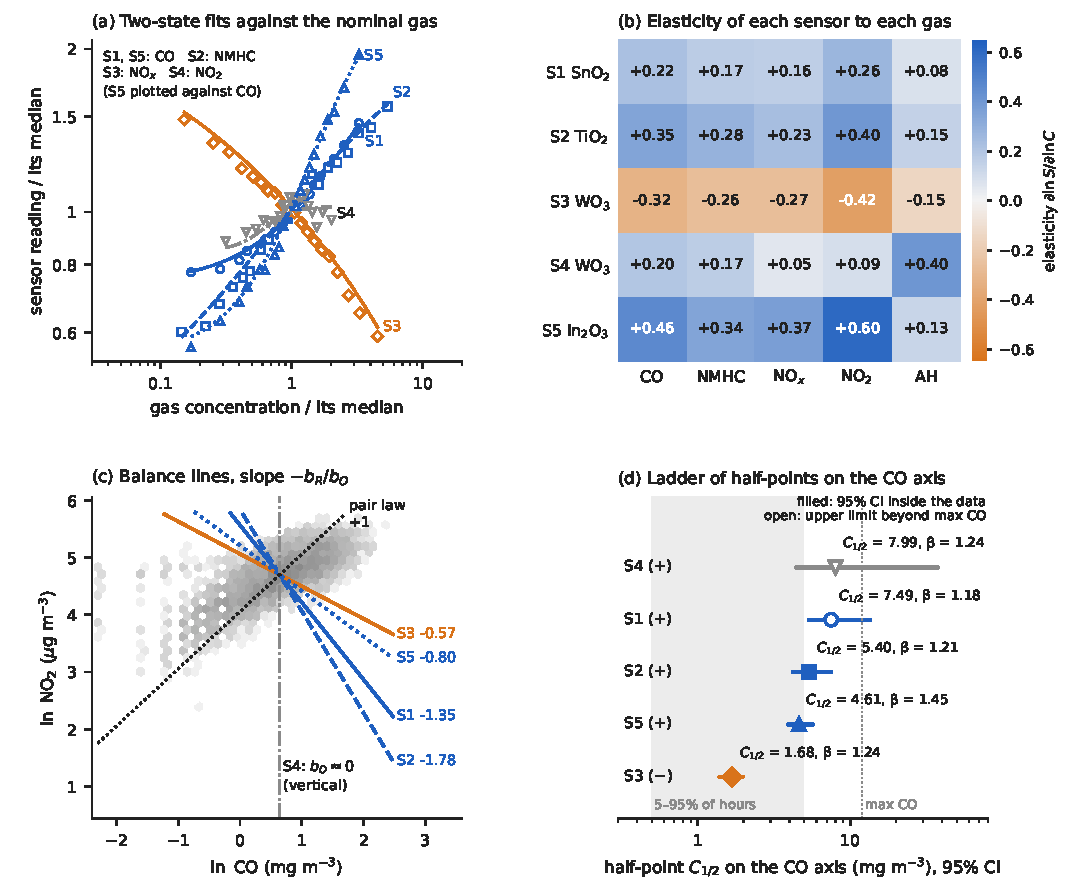
\includegraphics[width=\textwidth]{fig_sensor_ladder.pdf}
\caption{The sensor ladder of the UCI air-quality record (8991 hours with all five metal-oxide sensors present). Blue marks the sensors whose reading rises with the traffic gases (S1 tin oxide, S2 titania, S5 indium oxide), orange the tungsten-oxide sensor S3, which falls, and gray the tungsten-oxide sensor S4. (a) Binned medians (20 equal-count bins, open markers) of each sensor against its nominal reference gas, both normalised by their medians, with the fitted two-state law $S=S_\mathrm{lo}+(S_\mathrm{hi}-S_\mathrm{lo})/[1+(C_{1/2}/C)^\beta]$ (lines). Pairs: S1--CO, S2--NMHC (887 hours, March--April 2004), S3--NO$_x$, S4--NO$_2$, S5--CO (the record has no O$_3$ reference). (b) Log--log elasticities $\partial\ln S/\partial\ln C$ of the five sensors to CO, NMHC, NO$_x$, NO$_2$ and absolute humidity, from least-squares slopes over pairwise-present hours. (c) Balance lines in the $(\ln\mathrm{CO},\ln\mathrm{NO_2})$ plane, along which the fitted pair regression $\ln S=b_0+b_R\ln\mathrm{CO}+b_O\ln\mathrm{NO_2}+b_H\ln\mathrm{AH}$ gives a constant reading (slope $-b_R/b_O$, drawn through the median point). The dotted line is the slope $+1$ of the pair law with equal orders. The S4 line is vertical because its $b_O$ is null. Gray hexagons show the density of the 6941 jointly present hours. (d) The ladder: half-points $C_{1/2}$ of the two-state fits on the common CO axis, with day-block bootstrap 95\% intervals, ordered S3 ($1.68$ mg\,m$^{-3}$) $<$ S5 ($4.61$) $<$ S2 ($5.40$) $<$ S1 ($7.49$) $<$ S4 ($7.99$). Filled markers: interval inside the observed CO range. Open markers: upper end beyond the maximum hourly CO ($11.9$ mg\,m$^{-3}$, dotted). Shading: central 90\% of hourly CO. Labels give $\beta$.}
\label{fig:sensor}
\end{figure}

\subsection{Two gases and humidity}\label{sec:two}
The pair regression of \cref{sec:stat} reads the balance line of \cref{sec:mos} with CO as the reducing and NO$_2$ as the candidate oxidizing marker, over 6941 hours on 341 days. The regressors are collinear: the correlation of $\ln$CO and $\ln$NO$_2$ is $0.713$, of $\ln$CO and $\ln$AH $0.092$, and of $\ln$NO$_2$ and $\ln$AH $-0.308$; the variance inflation factors are $2.60$ ($\ln$CO), $2.85$ ($\ln$NO$_2$) and $1.41$ ($\ln$AH). \Cref{tab:pairreg} gives the coefficients, each with its 95\% interval on the line below.

\begin{table}[htbp]\centering
\caption{Pair regression $\ln S=b_0+b_R\ln\mathrm{CO}+b_O\ln\mathrm{NO_2}\,(+\,b_H\ln\mathrm{AH})$, 6941 hours, with the humidity term and without it (``no AH''). Second line of each entry: day-block bootstrap 95\% interval. The last-but-one column gives whether $b_R$ and $b_O$ have opposite signs, with the share of replicates in which they do.}\label{tab:pairreg}
\scriptsize\setlength{\tabcolsep}{3pt}
\begin{tabular}{@{}llccccll@{}}\toprule
sensor & model & $b_R$ (CO) & $b_O$ (NO$_2$) & $b_H$ (AH) & $-b_R/b_O$ & opposite signs & $R^2$\\\midrule
S1 & with AH & $+0.1610$ & $+0.1194$ & $+0.1019$ & $-1.348$ & no ($0.000$) & $0.7573$\\
 & & [$+0.1360$, $+0.1889$] & [$+0.0789$, $+0.1575$] & [$+0.0791$, $+0.1213$] & [$-2.422$, $-0.875$] & & \\
S2 & with AH & $+0.2662$ & $+0.1499$ & $+0.1614$ & $-1.776$ & no ($0.000$) & $0.8456$\\
 & & [$+0.2356$, $+0.3025$] & [$+0.1000$, $+0.2005$] & [$+0.1381$, $+0.1859$] & [$-3.017$, $-1.186$] & & \\
S3 & with AH & $-0.1692$ & $-0.2990$ & $-0.2130$ & $-0.566$ & no ($0.000$) & $0.7030$\\
 & & [$-0.2103$, $-0.1321$] & [$-0.3678$, $-0.2308$] & [$-0.2477$, $-0.1807$] & [$-0.895$, $-0.365$] & & \\
S4 & with AH & $+0.1835$ & $-0.0073$ & $+0.3829$ & $+25.0$ & $b_O$ null ($0.672$) & $0.7932$\\
 & & [$+0.1616$, $+0.2113$] & [$-0.0462$, $+0.0218$] & [$+0.3570$, $+0.4054$] & [$-274.5$, $+101.8$] & & \\
S5 & with AH & $+0.2839$ & $+0.3570$ & $+0.2071$ & $-0.795$ & no ($0.000$) & $0.7361$\\
 & & [$+0.2355$, $+0.3305$] & [$+0.2783$, $+0.4423$] & [$+0.1588$, $+0.2515$] & [$-1.173$, $-0.533$] & & \\
S1 & no AH & $+0.2016$ & $+0.0448$ & -- & $-4.50$ & no ($0.004$) & $0.7156$\\
 & & [$+0.1794$, $+0.2275$] & [$+0.0116$, $+0.0748$] & & [$-17.6$, $-2.35$] & & \\
S2 & no AH & $+0.3305$ & $+0.0317$ & -- & $-10.4$ & $b_O$ null ($0.092$) & $0.7969$\\
 & & [$+0.2970$, $+0.3682$] & [$-0.0123$, $+0.0737$] & & [$-174.6$, $+105.4$] & & \\
S3 & no AH & $-0.2540$ & $-0.1430$ & -- & $-1.777$ & no ($0.000$) & $0.6283$\\
 & & [$-0.2950$, $-0.2210$] & [$-0.1965$, $-0.0889$] & & [$-3.353$, $-1.117$] & & \\
S4 & no AH & $+0.3360$ & $-0.2878$ & -- & $\mathbf{+1.167}$ & yes ($1.000$) & $0.4650$\\
 & & [$+0.2944$, $+0.3855$] & [$-0.3650$, $-0.2201$] & & [$+1.040$, $+1.365$] & & \\
S5 & no AH & $+0.3664$ & $+0.2054$ & -- & $-1.784$ & no ($0.000$) & $0.6983$\\
 & & [$+0.3251$, $+0.4133$] & [$+0.1423$, $+0.2666$] & & [$-2.904$, $-1.239$] & & \\\bottomrule
\end{tabular}
\end{table}

\paragraph{What the regression gives.} In this urban record NO$_2$ rises with CO. Both are emitted by traffic (the correlation of their logarithms is $0.713$ over these hours), and NO$_2$ also follows the other reducing gases of the traffic plume (NMHC--NO$_2$ $0.823$, \cref{tab:collin}), so the CO and NO$_2$ coefficients carry the same sign on S1, S2, S3 and S5, in every bootstrap replicate, and their balance lines have negative slopes ($-1.348$, $-1.776$, $-0.566$ and $-0.795$). The oxidizing member of the surface pair is therefore not separable through NO$_2$ in this record. On S4 the NO$_2$ coefficient is null once humidity enters ($-0.0073$ [$-0.0462$, $+0.0218$]). Without the humidity term S4 has $b_R=+0.336$ and $b_O=-0.288$, of opposite sign in every replicate, and balance slope $+1.167$ [$1.040$, $1.365$], close to the slope $1$ of equal orders; the humidity term absorbs this structure because $\ln$NO$_2$ and $\ln$AH are correlated ($-0.308$) and S4 is dominated by humidity (elasticity $+0.404$, $R^2=0.521$). The same pattern holds in both halves of the year: only the warm-half $b_O$ of S1 touches zero ($+0.032$ [$-0.005$, $+0.059$]), and the $b_O$ of S4 is null in both halves (warm, 3056 hours: $-0.003$ [$-0.071$, $+0.040$]; cold, 3885 hours: $+0.036$ [$-0.021$, $+0.084$]).

\paragraph{The opposite-sign pair: CO against NO on S4.} Separating NO from NO$_2$ gives the regression $\ln S=b_0+b_1\ln\mathrm{CO}+b_2\ln\mathrm{NO}+b_3\ln\mathrm{NO_2}+b_4\ln\mathrm{AH}$ over 6940 hours (\cref{tab:no}); the regressor correlations are $0.738$ (CO--NO), $0.713$ (CO--NO$_2$) and $0.790$ (NO--NO$_2$).

\begin{table}[htbp]\centering
\caption{Regression with NO and NO$_2$ separated, 6940 hours. Second line: day-block bootstrap 95\% interval.}\label{tab:no}
\footnotesize
\begin{tabular}{@{}lccccc@{}}\toprule
sensor & CO & NO & NO$_2$ & AH & $R^2$\\\midrule
S1 & $+0.1441$ & $+0.0256$ & $+0.0896$ & $+0.1068$ & $0.7655$\\
 & [$+0.1187$, $+0.1728$] & [$+0.0141$, $+0.0369$] & [$+0.0622$, $+0.1166$] & [$+0.0867$, $+0.1272$] & \\
S2 & $+0.2575$ & $+0.0129$ & $+0.1356$ & $+0.1640$ & $0.8467$\\
 & [$+0.2227$, $+0.3001$] & [$-0.0012$, $+0.0251$] & [$+0.0935$, $+0.1810$] & [$+0.1396$, $+0.1875$] & \\
S3 & $-0.0986$ & $-0.1082$ & $-0.1704$ & $-0.2331$ & $0.7597$\\
 & [$-0.1285$, $-0.0710$] & [$-0.1263$, $-0.0884$] & [$-0.2213$, $-0.1297$] & [$-0.2612$, $-0.2055$] & \\
S4 & $+0.2286$ & $\mathbf{-0.0698}$ & $+0.0772$ & $+0.3702$ & $0.8248$\\
 & [$+0.2002$, $+0.2680$] & [$-0.0822$, $-0.0584$] & [$+0.0415$, $+0.1094$] & [$+0.3468$, $+0.3929$] & \\
S5 & $+0.2122$ & $+0.1099$ & $+0.2263$ & $+0.2274$ & $0.7672$\\
 & [$+0.1741$, $+0.2539$] & [$+0.0907$, $+0.1288$] & [$+0.1691$, $+0.2899$] & [$+0.1840$, $+0.2700$] & \\\bottomrule
\end{tabular}
\end{table}

The opposite-sign pair of the record appears on the tungsten-oxide sensor S4, as CO ($+0.229$) against NO ($-0.070$): its balance slope in the $(\ln\mathrm{CO},\ln\mathrm{NO})$ plane is $3.28$ [$2.90$, $3.73$], with opposite signs in all 2000 replicates. S3 falls with CO also when NO and NO$_2$ are held fixed ($-0.099$ [$-0.129$, $-0.071$]): its opposite direction is its own response to the reducing gas, not an effect of the co-emitted nitrogen oxides, and all its gas coefficients share one sign.

\paragraph{Humidity.} In \cref{tab:pairreg} the humidity coefficient $b_H$ has the sign of $b_R$ in all five sensors (S1 $+0.102$, S2 $+0.161$, S3 $-0.213$, S4 $+0.383$, S5 $+0.207$), and every interval excludes zero. The interaction model $\ln S=b_0+b_1\ln\mathrm{CO}+b_2\ln\mathrm{NO_2}+b_3\omega+b_4\,\omega\ln\mathrm{CO}+b_5\,\omega\ln\mathrm{NO_2}$, with $\omega=\ln\mathrm{AH}-\overline{\ln\mathrm{AH}}$, gives \cref{tab:hum}.

\begin{table}[htbp]\centering
\caption{Humidity interaction model. Second line: day-block bootstrap 95\% interval.}\label{tab:hum}
\scriptsize\setlength{\tabcolsep}{3.5pt}
\begin{tabular}{@{}lcccccc@{}}\toprule
sensor & $b_1$ & $b_2$ & $b_3$ & $b_4$ (CO$\times$AH) & $b_5$ (NO$_2\times$AH) & $R^2$\\\midrule
S1 & $+0.1646$ & $+0.1152$ & $+0.2020$ & $+0.0535$ & $-0.0270$ & $0.7625$\\
 & [$+0.1420$, $+0.1915$] & [$+0.0781$, $+0.1518$] & [$+0.0323$, $+0.3574$] & [$+0.0255$, $+0.0771$] & [$-0.0622$, $+0.0112$] & \\
S2 & $+0.2714$ & $+0.1452$ & $+0.6432$ & $+0.0648$ & $-0.1101$ & $0.8497$\\
 & [$+0.2380$, $+0.3051$] & [$+0.0992$, $+0.1926$] & [$+0.3736$, $+0.8841$] & [$+0.0087$, $+0.1079$] & [$-0.1663$, $-0.0473$] & \\
S3 & $-0.1838$ & $-0.2868$ & $-1.7370$ & $-0.1742$ & $+0.3452$ & $0.7362$\\
 & [$-0.2219$, $-0.1486$] & [$-0.3516$, $-0.2209$] & [$-2.0429$, $-1.4709$] & [$-0.2169$, $-0.1322$] & [$+0.2867$, $+0.4119$] & \\
S4 & $+0.1797$ & $-0.0037$ & $+0.0782$ & $-0.0494$ & $+0.0705$ & $0.7955$\\
 & [$+0.1584$, $+0.2079$] & [$-0.0448$, $+0.0260$] & [$-0.1934$, $+0.3135$] & [$-0.0996$, $-0.0079$] & [$+0.0187$, $+0.1331$] & \\
S5 & $+0.2898$ & $+0.3546$ & $+1.3845$ & $+0.0478$ & $-0.2578$ & $0.7494$\\
 & [$+0.2485$, $+0.3328$] & [$+0.2799$, $+0.4288$] & [$+0.9741$, $+1.7971$] & [$-0.0241$, $+0.1158$] & [$-0.3514$, $-0.1605$] & \\\bottomrule
\end{tabular}
\end{table}

Humidity is therefore not a common-mode term in this record. A common-mode term would cancel in $\varepsilon$ (\cref{prop:mos}), leave the gas elasticities unchanged and have no interactions. Instead absolute humidity shifts every reading in the direction of the reducing gas, which is the mass-action signature of an electron-donating co-adsorbate on the release side $\Phi_+$; it modulates the CO elasticity (interaction intervals exclude zero for S1, S2, S3 and S4) and the NO$_2$ elasticity (intervals exclude zero for S2, S3, S4 and S5).

\subsection{The benzene column is a transform of S2}\label{sec:benzene}
Over all 8991 present rows the Spearman correlation of S2 with C$_6$H$_6$(GT) is exactly $1$: sorted by S2, the benzene column never decreases. Least squares of $\ln\mathrm{C_6H_6}$ on $\ln(S_2-b)$ gives
\begin{equation}\label{eq:benzene}
\mathrm{C_6H_6}=1.23978\times10^{-4}\,(S_2-324.785)^{1.743158}\quad(\mu\mathrm g\,\mathrm m^{-3}),
\end{equation}
with maximum relative deviation $1.6\times10^{-15}$ and root-mean-square relative deviation $5.0\times10^{-16}$ at the least-squares values of the three parameters, over $S_2\in[383.25,2214.0]$ and $\mathrm{C_6H_6}\in[0.149,63.74]$; with the parameters rounded as printed, \eqref{eq:benzene} reproduces every value to a relative deviation of $4.5\times10^{-6}$. The column that the data-set page describes as the true hourly benzene concentration from the reference analyser is therefore a deterministic calibration of the titania sensor, not an independent measurement. It carries no information beyond S2: a model that predicts C$_6$H$_6$(GT) from the sensor channels recovers a known function of one of its own inputs, and because the transform is strictly increasing, every rank statistic of C$_6$H$_6$(GT) equals that of S2. We exclude it as a reference from all fits. Its form is exactly the power-law regime of \eqref{eq:twostate}, $S_2-S_\mathrm{lo}\propto C^{\beta}$ with $S_\mathrm{lo}=324.785$ and $\beta=1/1.743158=0.5737$; for comparison, the offset power law of S2 against CO has exponent $0.631$ with $S_\mathrm{lo}=372.6$ (\cref{tab:ladder2}).

\subsection{Summary of the sensor results}\label{sec:sensorsum}
Every sensor reading is a monotone, saturating function of the traffic-gas level, and the two-state logistic in $\ln C$ fits it better than the offset power law, with slopes $\beta=1.18$ to $1.45$ near first-order mass action. On the common CO axis the half-points form the ladder S3 ($1.68$) $<$ S5 ($4.61$) $<$ S2 ($5.40$) mg\,m$^{-3}$, identified inside the data and ordered in the same way in both halves of the year; the half-point of S1 ($7.49$) lies at the upper edge of the data, and that of S4 is not identified. S3 reads the opposite member of the pair, and it falls with CO also when NO and NO$_2$ are held fixed. Humidity is a release-side term, not a common-mode one. In this urban record NO$_2$ rises with CO, so the CO and NO$_2$ coefficients carry the same sign on S1, S2, S3 and S5 and the oxidizing member is not separable through NO$_2$; the opposite-sign pair is CO against NO on S4, with balance slope $3.28$ [$2.90$, $3.73$]. The benzene column is the provider's calibration of S2, in the power-law regime of the two-state law. The record has no O$_3$ reference, so S5 is read against CO.

\subsection{The same law in the giant planets}\label{sec:giants}
The same two-state law, reached through a mass-action balance between two opposing species as in \cref{prop:mos}, decides the top ice deck of the giant planets \cite{Planet}. There NH$_3$ and H$_2$S are consumed 1:1 by the NH$_4$SH lattice, and at every level where the solid coexists with the gas their mole fractions satisfy $x_{\mathrm N}x_{\mathrm S}=K(T)/P^2$, with $K(T)$ the NH$_4$SH dissociation constant in atm$^2$ and $P$ the pressure in atm. Write $\chi=\sqrt{K}/P$ for the common part and $x_{\mathrm N}=\chi e^{\varepsilon/2}$, $x_{\mathrm S}=\chi e^{-\varepsilon/2}$; then $x_{\mathrm N}x_{\mathrm S}=\chi^2$ holds identically, and the difference
\[
\Delta=x_{\mathrm N}-x_{\mathrm S}=2\chi\sinh(\varepsilon/2),\qquad\varepsilon=2\operatorname{arsinh}\frac{\Delta}{2\chi}=\ln\frac{x_{\mathrm N}}{x_{\mathrm S}},
\]
is conserved from the deep atmosphere upwards because the solid takes the two gases 1:1. The NH$_3$ share of the vapour is $\phi_{\mathrm N}=x_{\mathrm N}/(x_{\mathrm N}+x_{\mathrm S})=1/(1+e^{-\varepsilon})$, with $\phi_{\mathrm N}-\frac12=\frac12\tanh(\varepsilon/2)$. At the deck base the deep mole fractions $N$ and $S$ are still intact, so $\chi=\sqrt{NS}$ and $\varepsilon=\ln(N/S)$; above it $K$ falls on cooling, $\chi\to0$ and $\varepsilon\to\operatorname{sign}(\Delta)\cdot\infty$. The surviving member is $\operatorname{sign}(N-S)$, with mole fraction $|\Delta|$, and at $N=S$ neither survives. The deep N/S ratios are $4.73$ (Jupiter), $3.16$ (Saturn), $0.195$ (Uranus) and $0.170$ (Neptune) \cite{Planet}: the zero $N/S=1$ separates the gas giants, above whose NH$_4$SH deck NH$_3$ survives, from the ice giants, above whose deck H$_2$S survives. \Cref{tab:shared} sets the two systems side by side.

\begin{table}[htbp]\centering
\caption{One pair law on a sensor surface and at the NH$_4$SH deck of a giant planet.}\label{tab:shared}
\small
\begin{tabular}{@{}>{\raggedright\arraybackslash}p{0.2\textwidth}>{\raggedright\arraybackslash}p{0.37\textwidth}>{\raggedright\arraybackslash}p{0.37\textwidth}@{}}\toprule
 & metal-oxide sensor (\cref{sec:mos}) & NH$_4$SH deck \cite{Planet}\\\midrule
pair & a site holds the electron (O$^-$) or releases it & the surviving vapour is NH$_3$ or H$_2$S\\
balance & $\theta/(1-\theta)=\Phi_-/\Phi_+$ & $x_{\mathrm N}/x_{\mathrm S}=e^{\varepsilon}$ with $x_{\mathrm N}x_{\mathrm S}=K/P^2$\\
log-odds & $\varepsilon=\ln(\Phi_+/\Phi_-)=\beta_R\ln C_R-\beta_O\ln C_O+\mathrm{const}$ & $\varepsilon=2\operatorname{arsinh}(\Delta P/(2\sqrt K))$, equal to $\ln(N/S)$ at the base\\
occupancy & $1-\theta=1/(1+e^{-\varepsilon})$ & $\phi_{\mathrm N}=1/(1+e^{-\varepsilon})$\\
common part (cancels) & any factor common to $\Phi_+$ and $\Phi_-$ & $\chi=\sqrt K/P$, the geometric mean\\
zero & $C=C_{1/2}$: release flux equals trapping flux & $N=S$: neither gas survives\\
what the observer reads & which member holds the electron & which gas survives the deck\\\bottomrule
\end{tabular}
\end{table}

Both are instances of one mechanism: two opposing reactants compete for a shared partner, and mass action converts their ratio into an occupancy. On the sensor, reducing and oxidizing gases compete for the surface oxygen and its trapped electron; in the giants, NH$_3$ and H$_2$S are consumed together by the NH$_4$SH lattice. The sensor is an open steady state whose log-ratio is set by the ambient gases, with effective orders $\beta$ fitted at $1.18$ to $1.45$; the deck is a closed equilibrium titration with exact stoichiometric order $1$, whose log-ratio is driven to $\pm\infty$ by cooling. Plotted against $\varepsilon=\beta\ln(C/C_{1/2})$, with occupancy $(S-S_\mathrm{lo})/(S_\mathrm{hi}-S_\mathrm{lo})$, the binned readings of S1, S2, S3 and S5 collapse onto the single logistic $1/(1+e^{-\varepsilon})$ on which the four planets sit at their NH$_4$SH bases \cite{Planet}.


\section{The pair behind the periodic table}\label{sec:pair}
In his treatment of D\"obereiner's triads \cite{Dob1829} in atomic number, Scerri compared the medium-long and left-step (Janet) forms of the table and proposed placing hydrogen above fluorine to complete the triad H--F--Cl \cite{Scerri2008,Scerri2010,Scerri2022}. Comparing the two forms, he observed that the medium-long form is anomalous for groups~1 and~2 whereas the left-step form shows no exceptions \cite{Scerri2010}, and that in the left-step form triads consistently align with periods of equal length \cite{Scerri2022}. We give the arithmetic behind those observations. The pair appears twice: as the spin pair that fixes every capacity (this section), and as the pair of $Z$-gaps around the middle member of a triad (\cref{sec:triads}). The counts below come from exhaustive enumeration of the 118-element table generated from the Madelung order, and the property values from arithmetic on tabulated atomic data; every input is listed in \cref{sec:data}.

An orbital $(n,\ell,m_\ell)$ holds a spin pair, so a subshell holds $2(2\ell+1)$ electrons and a shell $\sum_{\ell<n}2(2\ell+1)=2n^2$. The Madelung rule orders subshells by $n+\ell$ and, within equal $n+\ell$, by $n$ \cite{AllenKnight}. It is an idealisation (several ground configurations, such as those of Cr and Cu, depart from it), but the block and group structure of the table follows it. Sorting the subshells $(n,\ell)$, $0\le\ell<n$, by $(n+\ell,n)$ gives
\[
1s\ 2s\ 2p\ 3s\ 3p\ 4s\ 3d\ 4p\ 5s\ 4d\ 5p\ 6s\ 4f\ 5d\ 6p\ 7s\ 5f\ 6d\ 7p .
\]
Filling these subshells in turn with $Z=1,\dots,118$ and starting a new period at every $ns$ subshell gives, by direct count, $L(1),\dots,L(7)=2,8,8,18,18,32,32$ and period ends $\Sigma(p)=\sum_{q\le p}L(q)=2,10,18,36,54,86,118$.

\begin{proposition}[period-pair law]\label{prop:pair}
Let $\kappa(m)$ be the capacity of all subshells with $n+\ell=m$. Then $\kappa(m)=2\lceil m/2\rceil^2$, and period $p$ consists of the $ps$ subshell together with the subshells with $n+\ell=p+1$ and $\ell\ge1$, so
\[
L(p)=\kappa(p+1)=2\left\lceil\tfrac{p+1}{2}\right\rceil^2 .
\]
In particular $L(2k)=L(2k+1)=2(k+1)^2$ for $k\ge1$, and $L(1)=2$ is the only length that occurs once.
\end{proposition}
\begin{proof}
With $n=m-\ell$ and $\ell\le n-1$, the admissible $\ell$ are $0,1,\dots,\lfloor (m-1)/2\rfloor$, so $\kappa(m)=2\sum_{\ell=0}^{\lfloor (m-1)/2\rfloor}(2\ell+1)=2(\lfloor (m-1)/2\rfloor+1)^2=2\lceil m/2\rceil^2$. The admissible range of $\ell$ is the same for $m=2k-1$ and $m=2k$, hence $\kappa(2k-1)=\kappa(2k)$. Within $n+\ell=m$ the rule orders subshells by increasing $n$, so the $s$ subshell ($n=m$) comes last. A period therefore extends from the $ps$ subshell (the last member of group $m=p$) through the subshells of group $m=p+1$ except its final $(p+1)s$: one $s$ subshell is exchanged for another, and $L(p)=\kappa(p+1)$. Then $L(2k)=\kappa(2k+1)=\kappa(2k+2)=L(2k+1)$.
\end{proof}

Reading the periods off the order displayed above confirms the subshell content of every period and $L(p)=\kappa(p+1)$ for $p=1,\dots,7$; the capacities are $\kappa(1),\dots,\kappa(9)=2,2,8,8,18,18,32,32,50$. Period~1 is unpaired because its partner would be period~0. The left-step table, whose rows are the groups $n+\ell=m$, has row lengths $2,2,8,8,18,18,32,32$ and no unpaired row; it is the form whose triads Scerri discusses \cite{Scerri2010,Scerri2022}. The same formula gives $L(8)=L(9)=50$ for the Madelung order continued past $Z=118$.

\section{Exact triads}\label{sec:triads}
\paragraph{Convention.} IUPAC group numbers 1--18, with H in group~1 and He in group~18. Group~3 is Sc, Y, Lu, Lr; La--Yb and Ac--No form the f-block and carry no group number. This is the assignment the Madelung order itself produces; the composition of group~3 is the subject of an IUPAC project, whose provisional report is \cite{ScerriG3}. Placing each element of the generated table by the rule stated after \cref{lem:align} (groups 1--2 counted from the left of the period, groups 3--18 from the right, the 28 f-block elements without a group) reproduces the IUPAC columns for all 18 groups; group~3 as Sc, Y, La, Ac is examined as a sensitivity check. A vertical triad is three consecutive members $Z_1<Z_2<Z_3$ of a group; it is exact if $Z_2-Z_1=Z_3-Z_2$. The $118-28=90$ elements with a group number form $90-18=72$ pairs of consecutive members and $90-2\cdot18=54$ vertical triads. Every group has exactly one member in each period from its first period onwards, so consecutive members lie in consecutive periods.

With $\Sigma(p)$ the last atomic number of period $p$ ($\Sigma(0)=0$), for $Z$ in period $p$ let $\pi_{\mathrm l}(Z)=Z-\Sigma(p-1)$ be its place counted from the left and $\pi_{\mathrm r}(Z)=\Sigma(p)-Z$ its place counted from the right.

\begin{lemma}[alignment]\label{lem:align}
If $Z$ lies in period $p$ and $Z'$ in period $p+1$, then
\[
Z'-Z=L(p)+\pi_{\mathrm l}(Z')-\pi_{\mathrm l}(Z)=L(p+1)-\bigl(\pi_{\mathrm r}(Z')-\pi_{\mathrm r}(Z)\bigr).
\]
Hence $Z'-Z=L(p)$ if and only if $\pi_{\mathrm l}(Z')=\pi_{\mathrm l}(Z)$, and $Z'-Z=L(p+1)$ if and only if $\pi_{\mathrm r}(Z')=\pi_{\mathrm r}(Z)$.
\end{lemma}
\begin{proof}
$Z'=\Sigma(p)+\pi_{\mathrm l}(Z')=\Sigma(p+1)-\pi_{\mathrm r}(Z')$ and $Z=\Sigma(p-1)+\pi_{\mathrm l}(Z)=\Sigma(p)-\pi_{\mathrm r}(Z)$; subtract.
\end{proof}

The s-block opens every period, so groups 1 and 2 have $\pi_{\mathrm l}=g$, with $g$ the group number; the p-block closes every period and, in periods 4--7, the d-block precedes it immediately, so groups 3--18 have $\pi_{\mathrm r}=18-g$ (He, at the end of period~1, has $\pi_{\mathrm r}=0$). Enumerating all 72 consecutive pairs confirms this: in groups 1--2 every pair has $\pi_{\mathrm l}(Z')=\pi_{\mathrm l}(Z)$ (left-aligned), in groups 3--18 every pair has $\pi_{\mathrm r}(Z')=\pi_{\mathrm r}(Z)$ (right-aligned), and no pair is neither.

\begin{corollary}\label{cor:gap}
For consecutive members $Z_1<Z_2$ of a group, with $Z_1$ in period $p_1$: in groups 1--2, $Z_2-Z_1=L(p_1)$, the length of the period of $Z_1$; in groups 3--18, $Z_2-Z_1=L(p_1+1)$, the length of the period of $Z_2$. Outside the s-block the gap equals the length of the period of $Z_1$ exactly when $L(p_1)=L(p_1+1)$, that is when $p_1\in\{2,4,6\}$ opens a pair of periods.
\end{corollary}
\begin{proof}
$Z_2$ lies in period $p_1+1$. In groups 1--2, $\pi_{\mathrm l}(Z_2)=\pi_{\mathrm l}(Z_1)=g$, and \cref{lem:align} gives $Z_2-Z_1=L(p_1)$; in groups 3--18, $\pi_{\mathrm r}(Z_2)=\pi_{\mathrm r}(Z_1)=18-g$, and it gives $Z_2-Z_1=L(p_1+1)$. By \cref{prop:pair}, $L(p_1)=L(p_1+1)$ with $1\le p_1\le6$ holds exactly for $p_1=2,4,6$.
\end{proof}
Of the 72 pairs, 49 have $Z_2-Z_1=L(p_1)$, 67 have $Z_2-Z_1=L(p_2)$ and 44 both (direct enumeration). These counts also follow by hand: the 11 pairs of groups 1--2 all have $Z_2-Z_1=L(p_1)$, and 6 of them (those with $p_1\in\{2,4,6\}$) also $L(p_2)$; the 61 pairs of groups 3--18 all have $Z_2-Z_1=L(p_2)$, and 38 of them (those with $p_1\in\{2,4,6\}$) also $L(p_1)$; hence $11+38=49$, $61+6=67$ and $6+38=44$; none outside groups 1--2 has $Z_2-Z_1=L(p_1)\ne L(p_2)$. Thus Li$\to$Na is $8=L(2)$, but Cl$\to$Br is $18=L(4)$, not $L(3)$. This is the arithmetic form of the asymmetry between groups 1--2 and the rest noted by Scerri \cite{Scerri2010}.

\begin{theorem}[exact triads]\label{thm:exact}
A vertical triad with members in periods $p,p+1,p+2$ is exact if and only if the two periods it spans have equal length: $L(p)=L(p+1)$ in groups 1--2 and $L(p+1)=L(p+2)$ in groups 3--18. By \cref{prop:pair} this holds if and only if $p$ is even in groups 1--2 and odd in groups 3--18, and then the common gap $s$ is the repeated length, $s\in\{8,18,32\}$.
\end{theorem}
\begin{proof}
By \cref{cor:gap} the two gaps are $L(p),L(p+1)$ in groups 1--2 and $L(p+1),L(p+2)$ in groups 3--18.
\end{proof}

\paragraph{Enumeration.} The table has 54 vertical triads; 27 are exact, exactly those spanning equal-length periods. The count follows from \cref{thm:exact}, with $p$ the period of $Z_1$: groups 1 and 2 have triads starting at $p=1,\dots,5$ and $p=2,\dots,5$, of which $p=2,4$ are exact ($2+2$); groups 3--12 start at $p=4,5$, of which $p=5$ is exact ($10$); groups 13--17 start at $p=2,\dots,5$, of which $p=3,5$ are exact ($10$); group 18 starts at $p=1,\dots,5$, of which $p=1,3,5$ are exact ($3$); in all $27$. By gap pair $(Z_2-Z_1,Z_3-Z_2)$ there are 3 triads at $(8,8)$, 8 at $(18,18)$ and 16 at $(32,32)$, against 1 at $(2,8)$, 8 at $(8,18)$ and 18 at $(18,32)$ (\cref{fig:triads}b). The exact triads are, for $s=8$: Li--Na--K, Be--Mg--Ca, He--Ne--Ar; for $s=18$: K--Rb--Cs, Ca--Sr--Ba, Al--Ga--In, Si--Ge--Sn, P--As--Sb, S--Se--Te, Cl--Br--I, Ar--Kr--Xe; for $s=32$: the ten d-block triads Y--Lu--Lr, Zr--Hf--Rf, \dots, Cd--Hg--Cn (groups 3--12), and In--Tl--Nh, Sn--Pb--Fl, Sb--Bi--Mc, Te--Po--Lv, I--At--Ts, Xe--Rn--Og.
D\"obereiner's four triads are all exact: Li--Na--K $(3,11,19)$ with $s=8$, and Ca--Sr--Ba $(20,38,56)$, Cl--Br--I $(17,35,53)$ and S--Se--Te $(16,34,52)$ with $s=18$.

\paragraph{Pair, merge and observer.} In an exact triad the middle element is the zero of the pair $(Z_1-Z_2,\,Z_3-Z_2)=(-s,+s)$, and the triad is $Z_2+\{-s,0,s\}$. \Cref{thm:exact} says when such a triad exists: two periods of equal length must follow each other, which is the period-pair law seen from inside a group. The gaps down a group are consecutive period lengths (group~1: $2,8,8,18,18,32$; group~18: $8,8,18,18,32,32$), so exact triads in one group meet end to end: K ends Li--Na--K and begins K--Rb--Cs; Ca, In, Sn, Sb, Te and I do the same in groups 2 and 13--17, and Ar and Xe link three exact triads in group~18. The shared end is the observer of the first triad and a member of the next: the chain is the merge of triads along a group.

\paragraph{Sensitivity and left-step form.} With group~3 as Sc, Y, La, Ac, group~3 becomes left-aligned; there are again 54 triads, 27 exact and no mismatch, with Sc--Y--La $(18,18)$ exact in place of Y--Lu--Lr. In the left-step table (rows $n+\ell=m$, each row ordered f, d, p, s from left to right, so that He heads the s-block column above Be) every column is right-aligned; it has 54 triads, 26 exact, and exactness again coincides with equal row lengths. It loses He--Ne--Ar, since He sits above Be and He--Be--Mg has gaps $(2,8)$. Moving H above F, as Scerri proposed \cite{Scerri2008}, adds the exact triad H--F--Cl $(8,8)$ and removes H--Li--Na, giving 27 of 54.

\begin{figure}[tb]
\centering
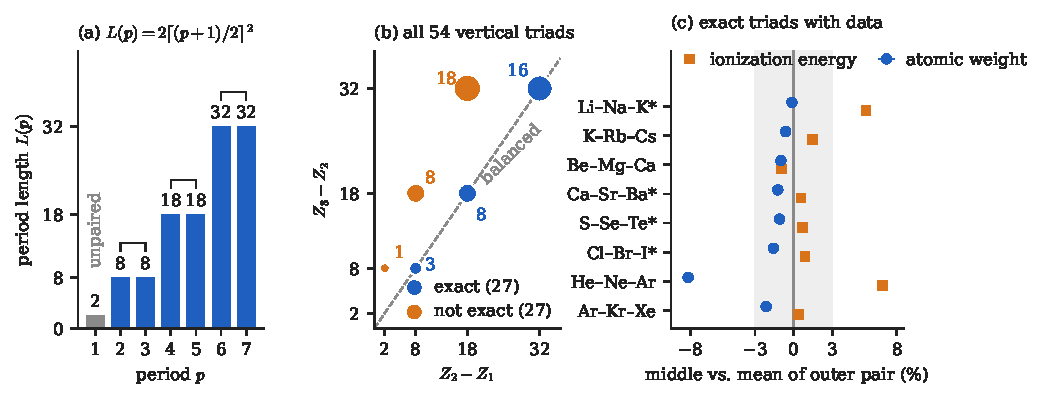
\includegraphics[width=\textwidth]{fig_chem2.pdf}
\caption{(a) Period lengths from the Madelung order; brackets join the equal pairs, and period~1 is unpaired. (b) The two $Z$-gaps of all 54 vertical triads; marker area grows with the number of triads (printed). Exact triads lie on the diagonal, at the repeated period lengths $8,18,32$. (c) Deviation of the middle member from the mean of the outer pair for the exact triads in groups 1, 2, 16, 17, 18 with data: standard atomic weight (circles; bars from the abridged uncertainties) and first ionization energy (squares). $^*$ marks D\"obereiner's triads; the band is $\pm3\%$.}
\label{fig:triads}
\end{figure}

\section{How far properties follow the balance}\label{sec:props}
For a property $x$ let $\eta=x_2/\bar x-1$, $\bar x=\frac12(x_1+x_3)$, be the deviation of the middle member from the mean of the outer pair. Standard atomic weights are the CIAAW abridged values \cite{CIAAW,Prohaska2022}; treating the printed uncertainties $u_i$ as independent standard uncertainties, first-order propagation gives
\[
u_\eta^2=\left(\frac{u_2}{\bar x}\right)^2+\left(\frac{x_2}{2\bar x^2}\right)^2(u_1^2+u_3^2),
\]
since $\partial\eta/\partial x_2=1/\bar x$ and $\partial\eta/\partial x_1=\partial\eta/\partial x_3=-x_2/(2\bar x^2)$. First ionization energies are those of the NIST Atomic Spectra Database \cite{NIST}, omitting values that the database marks as theoretical or estimated (printed in parentheses or brackets). All values used are listed in \cref{tab:data}. Te--Po--Lv, I--At--Ts and Xe--Rn--Og lack the data, so eight exact triads remain (\cref{tab:dev}, \cref{fig:triads}c).

\begin{table}[htbp]\centering
\caption{Deviation of the middle member from the mean of the outer pair, exact triads with data. $^*$: D\"obereiner's triads.}\label{tab:dev}
\small
\begin{tabular}{@{}lcrrc@{}}\toprule
triad & group, $s$ & $\eta_A$ (\%) & $\eta_{\mathrm{IE}}$ (\%) & IE between\\\midrule
Li--Na--K$^*$ & 1, 8 & $-0.13\pm0.13$ & $+5.61$ & yes\\
K--Rb--Cs & 1, 18 & $-0.62\pm0.01$ & $+1.45$ & yes\\
Be--Mg--Ca & 2, 8 & $-0.98\pm0.01$ & $-0.93$ & yes\\
Ca--Sr--Ba$^*$ & 2, 18 & $-1.22\pm0.01$ & $+0.57$ & yes\\
S--Se--Te$^*$ & 16, 18 & $-1.08\pm0.02$ & $+0.70$ & yes\\
Cl--Br--I$^*$ & 17, 18 & $-1.57\pm0.01$ & $+0.89$ & yes\\
He--Ne--Ar & 18, 8 & $-8.17\pm0.33$ & $+6.90$ & yes\\
Ar--Kr--Xe & 18, 18 & $-2.13\pm0.09$ & $+0.39$ & yes\\\bottomrule
\end{tabular}
\end{table}

\paragraph{Atomic weight.} The middle weight lies below the mean in all eight triads; for D\"obereiner's four, by $0.13$ to $1.57\%$. With $w_i=A_i/Z_i$ and $Z_2$ the exact mean, $Z_1=Z_2-s$ and $Z_3=Z_2+s$, so $2A_2-(A_1+A_3)=2w_2Z_2-w_1(Z_2-s)-w_3(Z_2+s)$, which is the identity
\[
2A_2-(A_1+A_3)=-Z_2\,(w_1+w_3-2w_2)-s\,(w_3-w_1).
\]
In the $s=18$ triads the second (trend) term, from the growth of $w$ with $Z$ (for example $2.058$, $2.310$, $2.417$ along K--Rb--Cs), lies between $-8.10$ and $-3.81$ and outweighs the curvature term. The largest deviation, He--Ne--Ar, reflects the weight of argon, dominated by $^{40}$Ar from the electron-capture branch of $^{40}$K (\cref{sec:k40}) \cite{GE}, which also places it above potassium ($39.95$ against $39.098$). Where the $Z$-pair is not balanced, neither is the weight: for the five non-exact triads in these groups with weights and no hydrogen (Na--K--Rb, Mg--Ca--Sr, O--S--Se, F--Cl--Br, Ne--Ar--Kr) the middle $Z$ lies $20.0$ to $23.8\%$ below the outer mean and the middle weight $23.2$ to $32.5\%$ below.

\paragraph{Ionization energy.} In all six exact triads of groups 1, 2, 16 and 17 and in both group-18 triads the middle energy lies strictly between the outer two. In seven of the eight it lies above the mean. Without a member from the first two periods the deviation is at most $1.45\%$ (K--Rb--Cs); with one it is $+5.61\%$ for Li--Na--K and $+6.90\%$ for He--Ne--Ar, and $-0.93\%$ for Be--Mg--Ca. The balance of $Z$ carries over to the ionization energy most closely below the second period, and least well at the top of the table, where the first member of a group differs most from its congeners: the first-member anomaly that Scerri weighs in his case for the left-step table \cite{Scerri2022}.

\paragraph{Where the balance breaks.} \emph{d-block contraction.} Ga, Ge, As, Se, Br and Kr follow the first filled 3d shell, whose electrons shield the nucleus poorly \cite{GE}. In all six exact triads with a 4p middle member, $\eta_{\mathrm{IE}}>0$ ($+1.92$, $+1.96$, $+2.52$, $+0.70$, $+0.89$, $+0.39\%$ for groups 13--18). For Ga the effect lifts its energy above that of Al, by $0.0135$ eV, so Al--Ga--In, exact in $Z$, is the one exact triad with data whose middle energy is not between the outer two. \emph{Relativistic effects.} In the non-exact triads Cu--Ag--Au and Zn--Cd--Hg the heaviest member has the highest ionization energy (Au exceeds Cu by $1.4992$ eV, Hg exceeds Zn by $1.0433$ eV), and in Rb--Cs--Fr and Sr--Ba--Ra the period-7 member lies above the period-6 member ($4.0727$ against $3.8939$ eV, $5.2784$ against $5.2117$ eV). This is the pattern of the relativistic stabilisation of $s$ shells in the heaviest elements \cite{Pyykko1988}. The exact triads Ag--Au--Rg and Cd--Hg--Cn lack measured energies for their heaviest members; Y--Lu--Lr, with $4.96(5)$ eV for Lr, gives $-2.91\%$.

\section{Horizontal triads and lanthanide-contraction pairs}\label{sec:explore}
Horizontal triads have $s=1$ and are exact in $Z$ by construction. Fe--Co--Ni gives $\eta_A=+2.91\%$, because cobalt ($58.933$) is heavier than nickel ($58.693$), and $\eta_{\mathrm{IE}}=+1.41\%$. Ru--Rh--Pd gives $-0.80\%$ and $-4.97\%$, and Os--Ir--Pt gives $-0.23\%$ and $+3.09\%$, with Ir above both neighbours.

For Ti--Zr--Hf and V--Nb--Ta the $Z$-gaps are $(18,32)$: the second gap exceeds the first by $14=2(2\cdot3+1)$, the capacity of the 4f subshell. The Shannon ionic radii (six-coordinate) are $0.605$, $0.72$, $0.71$~\AA{} for Ti$^{4+}$, Zr$^{4+}$, Hf$^{4+}$ and $0.54$, $0.64$, $0.64$~\AA{} for V$^{5+}$, Nb$^{5+}$, Ta$^{5+}$ \cite{Shannon}, as transcribed in \cite{ShannonDB}. The heavier two form a near-equal pair (ratio $0.986$ and $1.000$) although their weights differ by a factor of $1.957$ and $1.948$. This is the lanthanide contraction \cite{GE}. In these terms the radius triad collapses into a pair: one step from the first member and almost none between the heavier two, although in $Z$ the second step is the longer.

\section{Concluding remarks}\label{sec:summary}
In each case the chemically meaningful quantity is the difference of the pair: which configuration holds the electron, the net charge change of a branching, which level is the majority, whether two channels co-vary, which member holds a sensor surface's electron, and which element is the zero of a triad. The balance is unreachable (Na/K), unrealised, with a difference that two evaluations place $2.6$ combined standard uncertainties apart (${}^{40}$K), crossed at a finite temperature fixed by degeneracy (Al, $232.61$ K), manufactured by a shared code (absent measurements, where one coded correlation bounds how far the code sits from the data and the present-row moments reproduce it to $10^{-16}$), crossed at a concentration fixed by the equality of release and trapping (the sensor ladder, from $1.68$ to $7.49$ mg\,m$^{-3}$ of CO), or exact by counting (the 27 triads that span equal-length periods). The same law decides the gate of a membrane channel \cite{Neuro} and the top ice deck of a giant planet \cite{Planet}.

\paragraph{Outlook.} A record in which the oxidizing gas varies independently of the reducing ones, or one with an ozone reference, will place the oxidizing member and S5 on the same ladder and read the balance line of \cref{sec:mos} directly. The half-point analysis applies unchanged to any array of metal-oxide sensors recorded beside reference analysers.

\section{Data and sources}\label{sec:data}
All numbers not listed here are computed from these inputs by the formulas and methods stated in the text.
\begin{itemize}
\item \emph{Physical constants} (CODATA 2018 \cite{CODATA}): $k_B=8.617333262\times10^{-5}$ eV\,K$^{-1}$ (exact in the SI); second radiation constant $hc/k_B=1.438776877$ cm\,K; electron mass $m_e=5.48579909\times10^{-4}$ u (used only for the $1.5\times10^{-5}$ translational factor, with the mass numbers $23$ and $39$ for Na and K); molar gas constant $R=8.314462618$ J\,mol$^{-1}$\,K$^{-1}$ (for the NO$_2$ conversion factor).
\item \emph{Atomic data} (NIST Atomic Spectra Database, version 5.12 \cite{NIST}, accessed 24 September 2026; level designations as in \cite{SansonettiMartin}): first ionisation energies $\mathrm{IE(Na\,I)}=5.13907696(25)$ eV and $\mathrm{IE(K\,I)}=4.34066373(9)$ eV; ground levels Na $3s\,{}^2S_{1/2}$, K $4s\,{}^2S_{1/2}$, Na$^+$ and K$^+$ ${}^1S_0$; K\,I $4p\,{}^2P^\circ_{1/2}$ and ${}^2P^\circ_{3/2}$ at $12985.185724$ and $13042.896027\ \mathrm{cm^{-1}}$; Al\,I $3s^{2}3p\,{}^2P^\circ_{1/2}$ at $0$ and ${}^2P^\circ_{3/2}$ at $112.061\ \mathrm{cm^{-1}}$, next level $3s^{2}4s\,{}^2S_{1/2}$ at $25347.756\ \mathrm{cm^{-1}}$. Degeneracies are $g=2J+1$. The first ionization energies of the triad sections are listed in \cref{tab:data}.
\item \emph{Nuclear data for ${}^{40}$K}: isotopic abundance $0.000117(1)$ \cite{Meija}; ENSDF evaluation \cite{Chen}: $\beta^-$ $89.28(11)\%$, electron capture plus $\beta^+$ $10.72(11)\%$, $\beta^+$ $0.001\%$; KDK re-evaluation \cite{KDK} (Table~IV there, with the partial decay constants of \cite{Kossert}): $\beta^-$ $89.59(5)\%$, capture to the excited state of ${}^{40}$Ar $10.31(4)\%$, capture to the ground state $0.098\pm0.023\,(\text{stat})\pm0.010\,(\text{syst})\%$.
\item \emph{Standard atomic weights} $A_r$ (\cref{tab:data}): CIAAW abridged standard atomic weights 2024 \cite{CIAAW}, which are those of the 2021 report \cite{Prohaska2022} with the 2024 revisions for Gd, Lu and Zr; accessed 24 September 2026. Fr, Ra and Lr have no standard atomic weight, and the period-7 elements from Rg to Og have neither quantity. Numbers in parentheses are the printed uncertainties in units of the last digit. The molar mass of NO$_2$, $46.005$ g\,mol$^{-1}$, is formed from the abridged weights of N ($14.007$) and O ($15.999$).
\item \emph{Structural inputs} for \cref{sec:pair,sec:triads}: the capacities $2(2\ell+1)$ and the Madelung $(n+\ell,n)$ order \cite{AllenKnight}; atomic numbers $Z=1,\dots,118$; IUPAC group numbers 1--18 with H in group~1, He in group~18 and group~3 as Sc, Y, Lu, Lr \cite{ScerriG3}; D\"obereiner's four triads Li--Na--K, Ca--Sr--Ba, Cl--Br--I, S--Se--Te \cite{Dob1829,Scerri2008}. Everything in \cref{sec:pair,sec:triads} is computed from these by counting.
\item \emph{Ionic radii} (six-coordinate, \AA): Ti$^{4+}$ $0.605$, Zr$^{4+}$ $0.72$, Hf$^{4+}$ $0.71$, V$^{5+}$ $0.54$, Nb$^{5+}$ $0.64$, Ta$^{5+}$ $0.64$, from Table~1 of \cite{Shannon}, as transcribed in \cite{ShannonDB}.
\item \emph{Dataset} (\cref{sec:code,sec:sensor}): the UCI Air Quality data set \cite{UCI}, doi:10.24432/C59K5F, data-set page accessed 24 September 2026, introduced in \cite{DeVito}: hourly averaged responses of an array of five metal-oxide chemical sensors (PT08.S1 to PT08.S5) with reference-analyser concentrations and meteorological readings, recorded at road level in a polluted area of an Italian city, with missing values tagged $-200$. Part used: the spreadsheet workbook distributed with the data set, all 9357 dated rows (10 March 2004 18:00 to 4 April 2005 14:00), columns PT08.S1 to PT08.S5, CO(GT), NMHC(GT), C6H6(GT) (shown in \cref{sec:benzene} to be a transform of PT08.S2), NOx(GT), NO2(GT), T, RH and AH. The sensor identities, units and the absent-value code are those stated on the data-set page. Every statistic of \cref{sec:code,sec:sensor} is computed directly from this workbook; the semicolon-separated text version of the data set, which rounds the sensor channels to integers, is used only for the comparison stated in \cref{sec:code}.
\item \emph{Planetary N/S ratios} (\cref{sec:giants}): the nominal deep mole-fraction ratios $4.73$, $3.16$, $0.195$ and $0.170$ for Jupiter, Saturn, Uranus and Neptune, from the companion paper \cite{Planet}, which lists their observational sources.
\end{itemize}

\begin{table}[htbp]\centering
\caption{Atomic data used in \cref{sec:props,sec:explore}: standard atomic weights $A_r$ \cite{CIAAW} and first ionization energies IE \cite{NIST}.}\label{tab:data}
\footnotesize\setlength{\tabcolsep}{4pt}
\begin{tabular}{@{}lrll@{\hspace{14pt}}lrll@{}}\toprule
El. & $Z$ & $A_r$ & IE (eV) & El. & $Z$ & $A_r$ & IE (eV)\\\midrule
He & 2 & 4.0026(1) & 24.587389011(25) & Sr & 38 & 87.62(1) & 5.69486745(12)\\
Li & 3 & 6.94(6) & 5.391714996(22) & Y & 39 & 88.906(1) & 6.21726(10)\\
Be & 4 & 9.0122(1) & 9.322699(7) & Zr & 40 & 91.222(3) & 6.634126(5)\\
O & 8 & 15.999(1) & 13.618055(7) & Nb & 41 & 92.906(1) & 6.75885(4)\\
F & 9 & 18.998(1) & 17.42282(5) & Ru & 44 & 101.07(2) & 7.36050(5)\\
Ne & 10 & 20.180(1) & 21.564541(7) & Rh & 45 & 102.91(1) & 7.45890(5)\\
Na & 11 & 22.990(1) & 5.13907696(25) & Pd & 46 & 106.42(1) & 8.336839(10)\\
Mg & 12 & 24.305(2) & 7.646236(4) & Ag & 47 & 107.87(1) & 7.576234(25)\\
Al & 13 & 26.982(1) & 5.985769(3) & Cd & 48 & 112.41(1) & 8.993820(16)\\
Si & 14 & 28.085(1) & 8.15168(3) & In & 49 & 114.82(1) & 5.7863558(5)\\
P & 15 & 30.974(1) & 10.486686(15) & Sn & 50 & 118.71(1) & 7.343918(12)\\
S & 16 & 32.06(2) & 10.3600167(14) & Sb & 51 & 121.76(1) & 8.608389(12)\\
Cl & 17 & 35.45(1) & 12.967633(16) & Te & 52 & 127.60(3) & 9.009808(6)\\
Ar & 18 & 39.95(16) & 15.7596119(5) & I & 53 & 126.90(1) & 10.451236(25)\\
K & 19 & 39.098(1) & 4.34066373(9) & Xe & 54 & 131.29(1) & 12.1298437(15)\\
Ca & 20 & 40.078(4) & 6.1131549210(5) & Cs & 55 & 132.91(1) & 3.89390572743(17)\\
Fe & 26 & 55.845(2) & 7.9024681(12) & Ba & 56 & 137.33(1) & 5.2116646(12)\\
Co & 27 & 58.933(1) & 7.88101(12) & Lu & 71 & 174.97(1) & 5.425871(12)\\
Ni & 28 & 58.693(1) & 7.639878(17) & Hf & 72 & 178.49(1) & 6.825070(12)\\
Cu & 29 & 63.546(3) & 7.726380(4) & Ta & 73 & 180.95(1) & 7.549571(25)\\
Zn & 30 & 65.38(2) & 9.394197(6) & Os & 76 & 190.23(3) & 8.43823(20)\\
Ga & 31 & 69.723(1) & 5.9993020(12) & Ir & 77 & 192.22(1) & 8.96702(22)\\
Ge & 32 & 72.630(8) & 7.899435(12) & Pt & 78 & 195.08(2) & 8.95883(10)\\
As & 33 & 74.922(1) & 9.78855(25) & Au & 79 & 196.97(1) & 9.225554(4)\\
Se & 34 & 78.971(8) & 9.752368(6) & Hg & 80 & 200.59(1) & 10.437504(6)\\
Br & 35 & 79.904(3) & 11.81381(6) & Fr & 87 & -- & 4.0727411(11)\\
Kr & 36 & 83.798(2) & 13.9996055(20) & Ra & 88 & -- & 5.2784239(25)\\
Rb & 37 & 85.468(1) & 4.1771281(12) & Lr & 103 & -- & 4.96(5)\\\bottomrule
\end{tabular}
\end{table}

\paragraph{Contributions and use of AI.} The ideas, the research questions, the framework that links the fields, the choice of problems and the direction at every stage are the author's. The derivations, proofs, numerical checks, reference checks and drafting were produced with an AI system working under that direction, and were checked by separate AI review passes. Errors in that material are errors of the AI system, and any found will be corrected in a revised version. Publication-ethics policy (COPE, \emph{Authorship and AI tools}, 2023) does not allow an AI system to be listed as an author, so its use is declared here instead.

\begin{thebibliography}{99}\small
\bibitem{Dob1829} J.~W.~D\"obereiner, Versuch zu einer Gruppirung der elementaren Stoffe nach ihrer Analogie, \emph{Ann. Phys.} 91 (1829) 301--307. doi:10.1002/andp.18290910217
\bibitem{Scerri2008} E.~R.~Scerri, The role of triads in the evolution of the periodic table: past and present, \emph{J. Chem. Educ.} 85 (2008) 585--589. doi:10.1021/ed085p585
\bibitem{Scerri2010} E.~Scerri, Explaining the periodic table, and the role of chemical triads, \emph{Found. Chem.} 12 (2010) 69--83. doi:10.1007/s10698-010-9082-9
\bibitem{Scerri2022} E.~R.~Scerri, In praise of triads, \emph{Found. Chem.} 24 (2022) 285--300. doi:10.1007/s10698-022-09434-x
\bibitem{AllenKnight} L.~C.~Allen, E.~T.~Knight, The L\"owdin challenge: origin of the $n+\ell$, $n$ (Madelung) rule for filling the orbital configurations of the periodic table, \emph{Int. J. Quantum Chem.} 90 (2002) 80--88. doi:10.1002/qua.965
\bibitem{Chen} J.~Chen, Nuclear Data Sheets for $A=40$, \emph{Nucl. Data Sheets} 140 (2017) 1--376. doi:10.1016/j.nds.2017.02.001
\bibitem{KDK} L.~Hariasz et al.\ (KDK Collaboration), Evidence for ground-state electron capture of ${}^{40}$K, \emph{Phys. Rev. C} 108 (2023) 014327. doi:10.1103/PhysRevC.108.014327
\bibitem{Kossert} K.~Kossert et al., Activity standardization of two enriched ${}^{40}$K solutions for the determination of decay scheme parameters and the half-life, \emph{Appl. Radiat. Isot.} 188 (2022) 110362. doi:10.1016/j.apradiso.2022.110362
\bibitem{BarsanWeimar2001} N.~Barsan, U.~Weimar, Conduction model of metal oxide gas sensors, \emph{J. Electroceram.} 7 (2001) 143--167. doi:10.1023/A:1014405811371
\bibitem{MadouMorrison} M.~J.~Madou, S.~R.~Morrison, \emph{Chemical Sensing with Solid State Devices}, Academic Press, San Diego, 1989. ISBN 978-0-12-464965-1
\bibitem{YamazoeShimanoe} N.~Yamazoe, K.~Shimanoe, Theory of power laws for semiconductor gas sensors, \emph{Sens. Actuators B} 128 (2008) 566--573. doi:10.1016/j.snb.2007.07.036
\bibitem{DeVito} S.~De Vito, E.~Massera, M.~Piga, L.~Martinotto, G.~Di Francia, On field calibration of an electronic nose for benzene estimation in an urban pollution monitoring scenario, \emph{Sens. Actuators B} 129 (2008) 750--757. doi:10.1016/j.snb.2007.09.060
\bibitem{UCI} S.~De Vito, Air Quality [data set], UCI Machine Learning Repository, 2008, \url{https://archive.ics.uci.edu/dataset/360/air+quality} (accessed 24 September 2026). doi:10.24432/C59K5F
\bibitem{LittleRubin} R.~J.~A.~Little, D.~B.~Rubin, \emph{Statistical Analysis with Missing Data}, 3rd ed., Wiley, Hoboken NJ, 2019. doi:10.1002/9781119482260
\bibitem{SchaferGraham} J.~L.~Schafer, J.~W.~Graham, Missing data: our view of the state of the art, \emph{Psychol. Methods} 7 (2002) 147--177. doi:10.1037/1082-989X.7.2.147
\bibitem{Synth} A.~Singh, What a Zero Is: One Involution across Mathematics, Physics, Chemistry, Neuroscience, Computation and the Giant Planets, manuscript, 25 September 2026.
\bibitem{Neuro} A.~Singh, The Balanced Pair in Excitable Tissue: What a Membrane Reading Determines, and the Balanced Cortex, manuscript, 25 September 2026.
\bibitem{Planet} A.~Singh, The Four Giants as Balanced Pairs: Throats, Hearts, the Gas Ladder and the Interstellar Visitors, manuscript, 25 September 2026.
\bibitem{Algo} A.~Singh, Three Is Enough: Radix Economy, Balanced-Ternary Arithmetic and Ternary-Weight Networks, manuscript, 25 September 2026.
\bibitem{NIST} A.~Kramida, Yu.~Ralchenko, J.~Reader and NIST ASD Team, \emph{NIST Atomic Spectra Database} (version 5.12), National Institute of Standards and Technology, Gaithersburg MD, 2024, \url{https://physics.nist.gov/asd} (accessed 24 September 2026). doi:10.18434/T4W30F
\bibitem{SansonettiMartin} J.~E.~Sansonetti, W.~C.~Martin, Handbook of basic atomic spectroscopic data, \emph{J. Phys. Chem. Ref. Data} 34 (2005) 1559--2259. doi:10.1063/1.1800011
\bibitem{CODATA} E.~Tiesinga, P.~J.~Mohr, D.~B.~Newell, B.~N.~Taylor, CODATA recommended values of the fundamental physical constants: 2018, \emph{Rev. Mod. Phys.} 93 (2021) 025010. doi:10.1103/RevModPhys.93.025010
\bibitem{Meija} J.~Meija et al., Isotopic compositions of the elements 2013 (IUPAC Technical Report), \emph{Pure Appl. Chem.} 88 (2016) 293--306. doi:10.1515/pac-2015-0503
\bibitem{BarsanWeimar2003} N.~B\^arsan, U.~Weimar, Understanding the fundamental principles of metal oxide based gas sensors; the example of CO sensing with SnO$_2$ sensors in the presence of humidity, \emph{J. Phys.: Condens. Matter} 15 (2003) R813--R839. doi:10.1088/0953-8984/15/20/201
\bibitem{Kunsch} H.~R.~K\"unsch, The jackknife and the bootstrap for general stationary observations, \emph{Ann. Statist.} 17 (1989) 1217--1241. doi:10.1214/aos/1176347265
\bibitem{CIAAW} CIAAW (IUPAC Commission on Isotopic Abundances and Atomic Weights), Abridged standard atomic weights 2024, \url{https://www.ciaaw.org/abridged-atomic-weights.htm} (accessed 24 September 2026).
\bibitem{ScerriG3} E.~Scerri, Provisional report on discussions on group 3 of the periodic table, \emph{Chem. Int.} 43 (2021) 31--34. doi:10.1515/ci-2021-0115
\bibitem{Prohaska2022} T.~Prohaska, J.~Irrgeher, J.~Benefield, et al., Standard atomic weights of the elements 2021 (IUPAC Technical Report), \emph{Pure Appl. Chem.} 94 (2022) 573--600. doi:10.1515/pac-2019-0603
\bibitem{GE} N.~N.~Greenwood, A.~Earnshaw, \emph{Chemistry of the Elements}, 2nd ed., Butterworth-Heinemann, Oxford, 1997.
\bibitem{Pyykko1988} P.~Pyykk\"o, Relativistic effects in structural chemistry, \emph{Chem. Rev.} 88 (1988) 563--594. doi:10.1021/cr00085a006
\bibitem{Shannon} R.~D.~Shannon, Revised effective ionic radii and systematic studies of interatomic distances in halides and chalcogenides, \emph{Acta Cryst. A} 32 (1976) 751--767. doi:10.1107/S0567739476001551
\bibitem{ShannonDB} \emph{Database of Ionic Radii}, Imperial College London, data from R.~D.~Shannon (1976), \url{http://abulafia.mt.ic.ac.uk/shannon/} (accessed 24 September 2026).
\end{thebibliography}
\end{document}
